\documentclass[12pt,a4paper,openany,tikz]{book}

\usepackage[utf8]{inputenc}
\usepackage{cmap}
\usepackage{type1ec}
\usepackage[T1]{fontenc}
\usepackage{fancyhdr}
\usepackage{graphicx,epsfig}
\usepackage[slovene]{babel}
\usepackage{cite}
\usepackage{mathrsfs}
\usepackage{enumitem}
\usepackage{todonotes}
\usepackage{mdframed}
\usepackage{mathtools}
\usepackage{amsmath}
\usepackage{amsthm}
\usepackage{amssymb}
\usepackage{caption}
\usepackage{subcaption}
\usepackage[numbers]{natbib}
\usepackage{tikz}
\usetikzlibrary{graphs,graphs.standard,quotes}
\usepackage[a4paper,headheight=15pt]{geometry}
\renewcommand{\baselinestretch}{1.3}

\providecommand\mathplus{+}

\usepackage[pdftex,colorlinks,citecolor=black,filecolor=black,linkcolor=black,urlcolor=black,pagebackref,unicode]{hyperref}
\usepackage[acronym,toc,xindy]{glossaries}
\usepackage{tikz}


\theoremstyle{plain}
\newtheorem{thm}{Theorem}[chapter] % reset theorem numbering for each chapter

\theoremstyle{definition}
\newtheorem{defn}[thm]{Definicija} % definition numbers are dependent on theorem numbers
\newtheorem{exmp}[thm]{Primer} % same for example numbers

%Nastavitev glave in repa strani
\pagestyle{fancy}
\fancyhead{}
\renewcommand{\chaptermark}[1]{\markboth{\textsf{Poglavje \thechapter:\ #1}}{}}
\renewcommand{\sectionmark}[1]{\markright{\textsf{\thesection\  #1}}{}}
\fancyhead[RE]{\leftmark}
\fancyhead[LO]{\rightmark}
\fancyhead[LE,RO]{\thepage}
\fancyfoot{}
\renewcommand{\headrulewidth}{0.0pt}
\renewcommand{\footrulewidth}{0.0pt}

\DeclareMathAlphabet{\mathpzc}{OT1}{pzc}{m}{it}
\mdfsetup{nobreak=true}
\makeglossaries{}
%%%%%%%%%%%%%%%%%%%%%%%%%%%%%%%%%%%%%%%%%%%%%%%%%%%%%%%%%%%%%%%%
%% ccBeamer 0.1, 2007-07-02                                   %%
%% Written by Sebastian Pipping <webmaster@hartwork.org>      %%
%% ---------------------------------------------------------- %%
%% Licensed under Creative Commons Attribution-ShareAlike 3.0 %%
%% http://creativecommons.org/licenses/by-sa/3.0/             %%
%%%%%%%%%%%%%%%%%%%%%%%%%%%%%%%%%%%%%%%%%%%%%%%%%%%%%%%%%%%%%%%%


%% Images
\newcommand{\CcImageBy}[1]{%
	
\includegraphics[scale=#1]{creative_commons/cc_by_30.pdf}%
}
\newcommand{\CcImageCc}[1]{%
	
\includegraphics[scale=#1]{creative_commons/cc_cc_30.pdf}%
}
\newcommand{\CcImageDevNations}[1]{%
	
\includegraphics[scale=#1]{creative_commons/cc_dev_nations_30.pdf}%
}
\newcommand{\CcImageNc}[1]{%
	
\includegraphics[scale=#1]{creative_commons/cc_nc_30.pdf}%
}
\newcommand{\CcImageNd}[1]{%
	
\includegraphics[scale=#1]{creative_commons/cc_nd_30.pdf}%
}
\newcommand{\CcImagePd}[1]{%
	
\includegraphics[scale=#1]{creative_commons/cc_pd_30.pdf}%
}
\newcommand{\CcImageSa}[1]{%
	
\includegraphics[scale=#1]{creative_commons/cc_sa_30.pdf}%
}
\newcommand{\CcImageSampling}[1]{%
	
\includegraphics[scale=#1]{creative_commons/cc_sampling_30.pdf}%
}
\newcommand{\CcImageSamplingPlus}[1]{%
	
\includegraphics[scale=#1]{creative_commons/cc_sampling_plus_30.pdf}%
}


%% Groups
\newcommand{\CcGroupBy}[1]{% zoom
	\CcImageBy{#1}%
}
\newcommand{\CcGroupByNc}[2]{% zoom, gap
	\CcImageBy{#1}\hspace*{#2}\CcImageNc{#1}%
}
\newcommand{\CcGroupByNcNd}[2]{% zoom, gap
	\CcImageBy{#1}\hspace*{#2}\CcImageNc{#1}\hspace*{#2}\CcImageNd{#1}%
}
\newcommand{\CcGroupByNcSa}[2]{% zoom, gap
	\CcImageBy{#1}\hspace*{#2}\CcImageNc{#1}\hspace*{#2}\CcImageSa{#1}%
}
\newcommand{\CcGroupByNd}[2]{% zoom, gap
	\CcImageBy{#1}\hspace*{#2}\CcImageNd{#1}%
}
\newcommand{\CcGroupBySa}[2]{% zoom, gap
	\CcImageBy{#1}\hspace*{#2}\CcImageSa{#1}%
}
\newcommand{\CcGroupDevNations}[1]{% zoom
	\CcImageDevNations{#1}%
}
\newcommand{\CcGroupNcSampling}[2]{% zoom, gap
	\CcImageNc{#1}\hspace*{#2}\CcImageSampling{#1}%
}
\newcommand{\CcGroupPd}[1]{% zoom
	\CcImagePd{#1}%
}
\newcommand{\CcGroupSampling}[1]{% zoom
	\CcImageSampling{#1}%
}
\newcommand{\CcGroupSamplingPlus}[1]{% zoom
	\CcImageSamplingPlus{#1}%
}


%********************************************

\begin{document}

%********************************************

\newacronym{SaaS}{SaaS}{Software as a Service}
\newacronym{PaaS}{PaaS}{Platform as a Service}
\newacronym{IaaS}{IaaS}{Infrastructure as a Service}
\newacronym{API}{API}{Application programming interface}
\newacronym{DES}{DES}{Data encryption standard}
\newacronym{NIST}{NIST}{National Institute of Standards and Technology}
\newacronym{NBS}{NBS}{National Bureau of Standards}
\newacronym{AES}{AES}{Advanced encryption standard}
\newacronym{IV}{IV}{inicializacijski vektor}
\newacronym{ECB}{ECB}{Electronic Codebook}
\newacronym{CBC}{CBC}{Cipher Block Chaining}
\newacronym{CFB}{CFB}{Cipher Feedback}
\newacronym{OFB}{OFB}{Output Feedback}
\newacronym{RSA}{RSA}{Rivest-Shamir-Adleman}
\newacronym{IBE}{IBE}{Identity Based Encryption}
\newacronym{FE}{FE}{Functional encryption}
\newacronym{ABE}{ABE}{Attribute Based Encryption}
\newacronym{KP-ABE}{KP-ABE}{Key-policy attribute based encryption}
\newacronym{CP-ABE}{CP-ABE}{Ciphertext-policy attribute based encryption}
\newacronym{SSL}{SSL}{Secure Sockets Layer}
\newacronym{TLS}{TLS}{Transport Layer Security}
\newacronym{HTTPS}{HTTPS}{HTTP over TLS}


\newglossaryentry{MITM}
{
  name={napad vrinjenega napadalca},
  description={angl.\ man-in-the-middle/MITM attack}
}

\newglossaryentry{plaintext}
{
  name=čistopis,
  description={plaintext},
}

\newglossaryentry{tajnopis}
{
  name=tajnopis,
  description={ciphertext},
}

\newglossaryentry{enckey}
{
  name=šifrirni ključ,
  description={encryption key},
}

\newglossaryentry{otp}
{
  name=enkratni ščit,
  description={(angl.\ one time pad)},
}

\newglossaryentry{neizpodbitnost}
{
  name=preprečevanje tajenja,
  description={non-repudiation},
}

\newglossaryentry{zaupnost}
{
  name=zaupnost,
  description={Confidentiality},
}

\newglossaryentry{celovitost}
{
  name=celovitost,
  description={Integrity},
}

\newglossaryentry{availability}
{
  name=razpoložljivost,
  description={Availability},
}

\newglossaryentry{overjanje}
{
  name=overjanje,
  description={Authentication},
}

\newglossaryentry{avtorizacija}
{
  name=avtorizacija,
  description={Authorization},
}

\newglossaryentry{feistelovasifra}
{
  name=Feistlova šifra,
  description={encryption key},
}
\newglossaryentry{cold-boot-attack}
{
  name=Cold boot attack,
  description={Cold boot attack},
}

\newglossaryentry{deduplication}
{
  name=izločanje dvojnic,
  description={angl.\ deduplication},
}

\newglossaryentry{authority}
{
  name=upravnik,
  description={angl.\ authority},
}
\newglossaryentry{ciphertextindistinguishability}
{
  name=ciphertext indistinguishability,
  description={angl.\ ciphertext indistinguishability},
}

\newglossaryentry{rootkit}
{
  name=korenski komplet,
  description={angl.\ rootkit},
}

\newglossaryentry{secMPC}
{
  name=varno večstransko računanje,
  description={angl.\ secure multi-party computation},
}

\newglossaryentry{malleable}
{
  name=gnetljiv,
  description={angl.\ malleable},
}
\newglossaryentry{bootstrappable}
{
  name=samozagonska,
  description={angl.\ bootstrappable},
}
\newglossaryentry{hypervisor}
{
  name=hipernadzornik,
  description={angl.\ hypervisor},
}


%********************************************

% stran 1 med uvodnimi listi
\thispagestyle{empty}

\begin{center}
{\large
UNIVERZA V LJUBLJANI\\
FAKULTETA ZA RAČUNALNIŠTVO IN INFORMATIKO\\
}

\vspace{3cm}
{\LARGE Andraž Vrhovec}\\

\vspace{2cm}
\textsc{\textbf{\LARGE
Varnost podatkov v oblaku
}}

\vspace{2cm}
{ DIPLOMSKO DELO}\\
{ NA INTERDISCIPLINARNEM UNIVERZITETNEM ŠTUDIJU
}


\vspace{2cm}
{\Large Mentor: prof.\ dr.\ Aleksandar Jurišić}

\vfill
{\Large Ljubljana, 2016}
\end{center}

\newpage

\ \thispagestyle{empty}

\newpage

%********************************************

% stran 2 med uvodnimi listi
\thispagestyle{empty}

\vspace*{5cm}
{\small \noindent
To diplomsko delo je ponujeno pod licenco \textit{Creative Commons Priznanje avtorstva-Deljenje pod enakimi pogoji 2.5 Slovenija}
ali (po želji) novejšo različico.
To pomeni, da se tako besedilo, slike, grafi in druge sestavine dela kot tudi rezultati diplomskega dela lahko prosto distribuirajo,
reproducirajo, uporabljajo, dajejo v najem, priobčujejo javnosti in predelujejo, pod pogojem, da se jasno in vidno navede avtorja in naslov tega
dela in da se v primeru spremembe, preoblikovanja ali uporabe tega dela v svojem delu, lahko distribuira predelava le pod
licenco, ki je enaka tej.
Podrobnosti licence so dostopne na spletni strani \url{http://creativecommons.si/} ali na Inštitutu za
intelektualno lastnino, Streliška 1, 1000 Ljubljana.

\begin{center}% 0.66 / 0.89 = 0.741573033707865
  \CcImageCc{0.741573033707865}\hspace*{1ex}\CcGroupBySa{1}{1ex}
\end{center}
}

\begin{center}
\vfill
{\em
Besedilo je oblikovano z urejevalnikom besedil \LaTeX.
}
\end{center}

\newpage

\ \thispagestyle{empty}

\newpage

%********************************************

% stran 3 med uvodnimi listi
\thispagestyle{empty}

Namesto te strani {\bf vstavite} original izdane teme diplomskega dela s podpisom mentorja in dekana ter žigom fakultete, ki ga diplomant
dvigne v študentskem referatu, preden odda izdelek v vezavo!

\newpage

%********************************************

% stran 4 med uvodnimi listi je prazna
\ \thispagestyle{empty}

\newpage

%********************************************

% stran 5 med uvodnimi listi

\thispagestyle{empty}

\vspace{1cm}
\begin{center}
{\Large \textbf{IZJAVA O AVTORSTVU}}
\end{center}

\begin{center}
{\Large diplomskega dela}
\end{center}

\vspace{1cm}
Spodaj podpisani/-a \hspace{0.5cm} Andraž Vrhovec,

\vspace{0.5cm}
z vpisno številko \hspace{0.5cm} 63080117,

\vspace{1cm}
sem avtor diplomskega dela z naslovom:

\vspace{0.5cm}
Varnost v oblaku
\vspace{1.5cm}
S svojim podpisom zagotavljam, da:
\begin{itemize}
	\item sem diplomsko delo izdelal/-a samostojno pod mentorstvom

	prof.\ dr.\ Aleksandar Jurišić

	\item	so elektronska oblika diplomskega dela, naslov (slov., angl.), povzetek (slov., angl.) ter ključne besede (slov., angl.) identični s tiskano obliko diplomskega dela
	\item soglašam z javno objavo elektronske oblike diplomskega dela v zbirki ``Dela FRI''.
\end{itemize}

\vspace{1cm}
V Ljubljani, dne \today \hspace{1cm} Podpis avtorja/-ice:

\newpage

%*******************************************

% stran 6 med uvodnimi listi je prazna pri dvostranskem tiskanju
\ \thispagestyle{empty}

\newpage

%********************************************

% stran 7 med uvodnimi listi

\chapter*{Zahvala}

\thispagestyle{empty}
Mogoče


\newpage

%********************************************

% stran 8 med uvodnimi listi je prazna pri dvostranskem tiskanju
\ \thispagestyle{empty}

\newpage

%********************************************

% stran 9 med uvodnimi listi
% \thispagestyle{empty}
%
% $\;$
%
% \vspace{5cm}
% \hfill{\Large \em Morebitno posvetilo\/ }
% \thispagestyle{empty}

\newpage

% stran 10 med uvodnimi listi je prazna pri dvostranskem tiskanju

\ \thispagestyle{empty}

\newpage

%********************************************

\renewcommand\thepage{}
\tableofcontents
\renewcommand\thepage{\arabic{page}}

\thispagestyle{empty}


%********************************************

\thispagestyle{empty}
\glsaddall{}
\printglossary[title=Slovarček]{}
\printglossary[type=\acronymtype,title=Seznam kratic in okrajšav] % prints just the list of acronyms

%\cleardoublepage

\clearpage{\pagestyle{empty}\cleardoublepage}

%********************************************
%začno se glavni listi, ki so numerirani z arabskimi stevilkami

\chapter*{Povzetek}

\addcontentsline{toc}{chapter}{Povzetek}

\todo[inline]{Napiši povzetek}

\vspace{1.3cm}
\noindent
{\large \bf Ključne besede:}

\vspace{0.5cm}
\noindent
diploma, oblak, varnost, kriptografija, kriptosistemi

\vspace{1cm}
\noindent
{\large \bf Keywords:}

\chapter*{Abstract}

\addcontentsline{toc}{chapter}{Abstract}

Povzetek naj bo napisan v angleškem jeziku.

\vspace{1.3cm}
\noindent
{\large \bf Keywords:}

\vspace{0.5cm}
\noindent
diploma, cloud, security, cryptography, cryptosystem


%********************************************
\setcounter{page}{1}
\pagenumbering{arabic}
\chapter{Uvod}

V zadnjih letih smo priča bliskovitemu porastu popularnosti računalništva v oblaku. Gartner je v začetku leta 2015 uvrstil računalništvo v oblaku med 10 strateško najpomembnejših tehnoloških trendov, ki bodo krojili prihodnost. Oblak nam omogoča udobno, cenovno ugodno delo kadarkoli in kjerkoli, tudi zunaj pisarne, saj je vse kar potrebujemo internetni dostop in računalnik ali telefon.

Računalništvo v oblaku je posledica razvoja več različnih tehnologij, ki so skupaj omogočile cenovno učinkovite rešitve, ki so hkrati preproste za uporabo. Končni uporabniki uporabljajo oblak, ker je preprost za uporabo ter omogoča dostop do podatkov kjerkoli in kadarkoli. Na drugi strani vedno več podjetji v želji, da znižajo stroške poslovanja in povečajo sposobnost prilagajanja zahtevam trga, seli svoje poslovanje v oblak. Posledica tega premika je selitev podatkov iz fizičnih nosilcev, ki so bili tradicionalno v lasti iste osebe kot podatki, v oblak. To pomeni, da varnost hrambe svojih podatkov zaupamo tretjim osebam. Za veliko ljudi in manjših podjetji je skrb za varnost podatkov (pre)velik zalogaj, ki zahteva ustrezno tehnično izobrazbo, strojno opremo in prostor. Kadar hranimo podatke v oblaku, nič od tega ni potrebno, saj nam vse to zagotavlja ponudnik storitev v oblaku v zameno za mesečno naročnino.

V kolikor vseeno ne želimo vseh svojih podatkov zaupati ponudniku storitve, pa nam kriptografija ponuja nekaj rešitev, kako zavarovati podatke pred nepooblaščenimi očmi. Posebej zanimive so metode šifriranja podatkov, saj zagotavlja zaščito pred širokom naborom groženj, ki jih bomo spoznali kasneje.  V nadaljevanju bomo najprej pogledali, kaj se skriva pod pojmoma ``oblak'' in ``varnost'', nato pa se posvetili kriptografskim metodam varovanja podatkov.

\section{Kaj je oblak?}
\label{sec:Kaj je oblak?}


Priljubljen internetni rek gre nekako takole: “there is no cloud, just someone else's computer”. Oblak ni nič drugega kot skupek velikega števila računalnikov, ki niso v lasti uporabnika storitve v oblaku, morda niso niti v lasti ponudnika storitve, ampak jih ta najema pri tretjem ponudniku. Pojem oblak je le krovni izraz za nove načine ponudbe in uporabe storitev, zato ga moramo podrobneje razdelati in razložiti.

NIST opredeli oblak kot: ``Računalništvo v oblaku je model, ki omogoča vseprisoten preprost dostop na zahtevo do skupnih računalniških virov (omrežja, strežniki, pomnilniški mediji, aplikacije in storitve), ki so lahko hitro pridobljeni ali sproščeni z minimalnim trudom in popolnoma samodejno, brez posredovanja ponudnika storitve. Model oblaka sestavlja pet ključnih lastnosti, trije nivoji storitve in štirje tipi oblakov.''~\cite{mell2011nist}

\subsection{Lastnosti oblaka}
\label{sub:Lastnosti oblaka}

\begin{description}[style=nextline]
   \item[Storitev na zahtevo] Stranka lahko pridobi nove vire v oblaku po potrebi, lahko tudi popolnoma samodejno, brez človeškega posredovanja.

   \item[Širok dostop preko omrežja] Zmogljivosti oblaka so na voljo preko omrežja in do njih lahko dostopamo preko standardnih mehanizmov, kar omogoča dostop praktično katerekoli naprave, ki se je zmožna povezati v omrežje (telefoni, tablice, računalniki,~\ldots).

   \item[Uporaba skupnih virov] Ponudnikovi fizični viri so združeni v bazen virov iz katerega stranke dobijo virtualizirane vire. Virtualizirani vir lahko prosto prehaja med fizičnimi gostitelji, zato težko govorimo o točni lokaciji vira.

   \item[Bliskovita prožnost] Uporabnik lahko preprosto poveča ali zmanjša zmogljivosti virov, ki jih uporablja, glede na potrebe. Uporabnik ima pogosto občutek, da so mu na voljo neomejene zmogljivosti.

   \item[Merjenje porabe in obračun glede na porabo virov]  Oblačni sistemi samodejno nadzirajo in optimizirajo porabo virov z metrikami (poraba prostora, pasovne širine, procesorskega časa~\ldots). Poraba virov se nadzira, kontrolira in poroča, kar omogoča transparentnost za ponudnika in uporabnika.
\end{description}

\subsection{Nivoji storitve}
\label{sub:Nivoji storitve}

\begin{description}[style=nextline]
	\item[\gls{SaaS}] Ponudnik storitev uporabniku omogoča uporabo njegove aplikacije, ki teče v oblaku. Aplikacija je dosegljiva iz različnih naprav, preko recimo spletnega brskalnika ali aplikacijskega vmesnika (API). Uporabnik nima nadzora nad infrastrukturo, na kateri teče aplikacija (omrežje in strežniki), kot tudi ne nad samo aplikacijo (z izjemo konfiguracije aplikacije).

	\item[\gls{PaaS}] Ponudnik storitev uporabniku ponuja platformo, na katero uporabnik namesti lastne ali kupljene aplikacije, ki so prilagojene za delovanje v oblaku. Tudi tu uporabnik nima nadzora nad infrastrukturo na kateri teče aplikacije, ima pa popolni nadzor nad aplikacijo.

	\item[\gls{IaaS}] Ponudnik uporabniku omogoča postavitev osnovnih gradnikov računalniškega sistema (procesiranje, hramba podatkov, omrežje …) iz katerih lahko uporabnik sestavi kar želi. Uporabnik sicer nima nadzora nad spodaj ležečo fizično infrastrukturo, vendar ima ves nadzor nad virtualiziranimi viri ki jih pridobi.
\end{description}

\subsection{Tipi oblakov}
\label{sub:Tipi oblakov}
\begin{description}[style=nextline]
	\item[Zasebni oblak] Vsa infrastruktura je namenjena uporabi znotraj ene organizacije, ki je sestavljena iz več delov. Upravljanje, vzdrževanje in lastništvo so lahko v domeni iste organizacije, tretje osebe ali kombinacije obojega. Lokacija sistema je lahko v prostorih organizacije ali pa izven njih.

	\item[Skupni oblak] Infrastruktura je namenjena uporabi s strani skupnosti organizacij, ki imajo skupne zahteve ali skupen cilj. Upravljanje, vzdrževanje in lastništvo je lahko v domeni ene ali večih organizacij znotraj skupnosti, tretje osebe ali kombinacije obojega. Lokacija sistema je lahko v prostorih ene od organizacij ali pa izven njih.

	\item[Javni oblak] Infrastruktura je namenjena uporabi s strani vseh. Ponudnik je lahko zasebno podjetje, izobraževalna ustanova ali vladna agencija. Infrastruktura se ponavadi nahaja na lokaciji ponudnika.

  \item[Hibridni oblak] Hibridni oblak je kombinacija dveh ali več tipov oblakov iz prvih treh točk (zasebni, javni, skupni). Oblaka sta sicer fizično ločena, vendar skupni standardi in tehnologije omogočajo preprosto prehajanje aplikacij in podatkov iz enega v drugega.
\end{description}

\section{Kaj je varnost?}
\label{sec:Kaj je varnost?}


Varnost je širok pojem, ki ga v kontekstu računalništva lahko razdelimo na tri dele. Računalniško varnost (computer security), informacijsko varnost (information security) in varovanje podatkov (information assurance).

\begin{description}
	\item[Računalniška varnost] se ukvarja z varovanjem računalniških sistemov, od strojne opreme preko programske opreme do podatkov, ki se procesirajo na tej strojni opremi. Naloga računalniške varnosti je zagotoviti integriteto, dostopnost in zaupnost vseh sestavnih delov računalniškega sistema.

  \item[Informacijska varnost] se ukvarja z varovanjem podatkov, ki se obdelujejo in shranjujejo v informacijskih sistemih. Njena naloga je zaščititi podatke pred nepooblaščenim dostopom, uporabo, spreminjanjem in uničenjem z ciljem zagotavljanja integritete, dostopnosti in zaupnosti podatkov.

  \item[Varovanje podatkov] se ukvarja z varovanjem podatkov in upravljanjem tveganj povezanih z uporabo, prenosom in procesiranjem podatkov s ciljem zagotavljanja integritete, dostopnosti, zaupnosti in neizpodbitnosti podatkov.
\end{description}

Iz teh opisov lahko razberemo ključne lastnosti varnega računalniškega sistema. V literaturi se te ključne tri lastnosti imenujemo CIA triad, kjer je CIA angleška kratica za ključne 3 lastnosti:



\begin{description}
\item[\Gls{zaupnost} (confidentiality)] pomeni zasebnost podatkov. Ukrepi, ki zagotavljajo zaupnost podatkov so usmerjeni k preprečevanju dostopa nepooblaščenih oseb. Pogosti mehanizmi, ki se uporabljajo za zagotavljanje zaupnosti podatkov so: zaščita z uporabniškim imenom in geslom, dvostopenjska overitev (two-factor auth), biometrična overitev in šifriranje podatkov.

\item[\Gls{celovitost} (integrity)] pomeni ohranjanje točnosti in pravilnosti podatkov. Ukrepi, ki zagotavljajo celovitost podatkov, preprečujejo nepooblaščenim osebam spreminjanje podatkov med prenosom ali v mirovanju. Omogočajo sledenje spremembam podatkov skozi zgodovino (revizijska sled), obnovitev podatkov iz varnostne kopije, v primeru, da pride do nepooblaščene spremembe. Mehanizmi, ki zagotavljajo celovitost podatkov so: nadzor dostopa in zgoščevalne funkcije ter digitalni podpisi.

\item[\Gls{availability} (availability)] pomeni, da so podatki vedno na voljo pooblaščenim osebam. Glavni vzrok nerazpoložljivosti so programske in strojne napake ter napadi zavrnitve storitve (denial of service). Razpoložljivost podatkov se zagotavlja z rednim vzdrževanjem strojne in programske opreme in s posebnimi ukrepi za preprečevanje napadov zavrnitve storitve.

\end{description}

Poleg treh ključnih lastnosti, ki jih najdemo zgoraj, je Meier~\cite{meier2003improving} identificiral še tri lastnosti, to so:

\begin{description}

\item[\Gls{overjanje}] identificira vir podatka oziroma izvor operacije, ki je lahko človek ali računalnik, in zagotovi, da je res tisti, za katerega se izdaja.

\item[\Gls{avtorizacija}] nadzira dostop do virov glede na pravila sistema in dodeljene pravice. Avtorizacijski mehanizmi uporabnikom preprečujejo, da bi presegli svoja pooblastila.

\item[\Gls{neizpodbitnost}] onemogoča uporabniku, da izpodbija oziroma zanika neko dejanje ali veljavnost pogodbe.

\end{description}

Vse zgoraj naštete lastnosti so splošne lastnosti varnosti in zato seveda tičejo tudi računalništva v oblaku. Pri uporabi storitev v oblaku, bi morali najbolj izpostaviti vprašanje varnosti podatkov, saj le te zaupamo v hrambo ponudniku storitve.

\chapter{Varnostna tveganja v oblaku}

Zaradi vse večje priljubljenosti storitev v oblaku in posledično ogromne količine podatkov, s katerimi razpolagajo ponudniki storitev v oblaku, so ti vedno pogosteje tarča napadov kriminalnih združb. Za sisteme, ki tečejo “v oblaku”, je značilno, da navzven delujejo kot en strežnik, v resnici pa tečejo na velikem številu strežnikov, ki so med seboj povezani. To pomeni da morebitni vdor v samo en strežnik napadalcu omogoča dostop na ostale strežnike, ki tečejo znotraj istega sistema. Če si sistem predstavljamo kot trdnjavo, to pomeni, da je večina zaščitnih mehanizmov skoncentrirana na obrobju, na obzidju trdnjave. Če uspemo to obzidje predreti na samo enem delčku, se lahko več ali manj prosto sprehajamo znotraj trdnjave. Pred pojavom storitev v oblaku je bilo znotraj enega obzidja le nekaj strežnikov, zato je bilo obzidje majhno in ga je bilo lažje vzdrževati. Sistem, na katerem teče storitev v oblaku pa je lahko sestavljen iz več tisoč strežnikov, kar pomeni, da se velikost obzidja močno poveča, veliko obzidje pa je tudi težko vzdrževati, zato se v njem hitro pojavijo razpoke.

Druga stvar, ki dela sisteme v oblaku zanimive za napadalce, je koncentracija podatkov. V primeru vdora v klasični strežnik, napadalec dobi dostop do veliko manjše količine podatkov kot ob vdoru v oblačni sistem. Razlog je preprost, saj na en sam strežnik fizično ni mogoče shraniti toliko podatkov, kot na sistem, ki je sestavljen iz tisočih strežnikov.

Ranljivost računalniškega sistema je lastnost, zaradi katere je ogroženo njegovo delovanje in varnost podatkov, ki jih vsebuje. Storitve, ki delujejo v oblaku,  podedujejo vse ranljivosti, ki jih imajo klasični računalniški sistemi, zaradi posebnih lastnosti oblaka, pa obstaja se nekaj groženj, specifičnih za storitve v oblaku:

\begin{description}[style=nextline]

\item[Nedovoljen dostop do upraviteljskega in programskega vmesnika] narava storitev v oblaku zahteva da so upraviteljski vmesniki dostopni preko interneta široki množici uporabnikov, kar posledično pomeni da so ti vmesniki izpostavljeni napadom preko interneta.

\item[Ranljivosti Internetnega protokola] Ena ključnih lastnosti oblaka je tudi široka dostopnost preko standardiziranih protokolov, zato je potrebno ko govorimo o varnosti v oblaku upoštevati tudi vse ranljivosti uporabljenih protokolov, kot je recimo \gls{MITM}.

\item[Ranljivosti obnovitve podatkov] Zaradi uporabe skupnih virov, ki je ena ključnih lastnosti oblaka, se lahko en fizični nosilec podatkov, ki je prej pripadal enemu uporabniku, kasneje dodeli drugemu uporabniku. Če pred tem ne poskrbimo za varen izbris podatkov, lahko drug uporabnik obnovi izbrisane podatke z nosilca in tako pride do razkritja podatkov.

\item[Izogibanje merjenju in plačilu] Storitve v oblaku se običajno plačujejo po porabi. Prav tako za začetek uporabe storitve praviloma vnesemo samo nekaj osnovnih podatkov in številko kreditne kartice. Napadalec nam lahko predloži ukradene podatke ali spreminja podatke o porabi, da se izogne plačilu.

\end{description}

\section{Izzivi na področju varnosti v oblaku}
\label{sec:Izzivi na področju varnosti v oblaku}

\subsection{Razkritje podatkov}
\label{sub:Razkritje podatkov}

O razkritju podatkov govorimo v primeru, da se občutljivi in zaupni podatki znajdejo na očeh nepooblaščenih oseb.  To se lahko zgodi kot posledica usmerjenega napada ali zaradi človeške napake, napake v aplikaciji ali slabih varnostnih mehanizmov aplikacije. Primeri zaupnih podatkov, ki so pogosto tarča napadov so: zdravstveni podatki, finančni podatki, osebno določljivi podatki, poslovne skrivnosti in intelektualna lastnina.

Razkritje podatkov je stara in vseprisotna grožnja v vseh računalniških sistemih, vendar je zaradi prej omenjene koncentracije podatkov ta grožnja v oblačnih sistemih še večja.

Obseg škode, ki ga povzroči razkritje podatkov, je odvisen od občutljivosti podatkov, ki so bili odtujeni. V veliko državah po svetu obstajajo zakoni in predpisi, ki podjetja ki hranijo določene tipe občutljivih podatkov, obvezuje k določenim standardom zaščite. V primeru, da pride do razkritja podatkov, lahko odgovorno podjetje doleti denarna kazen ali celo kazenska ovadba. Poleg škode, ki je bila povzročena z razkritjem podatkov in morebitno denarno kaznijo, so tu še stroški preiskave incidenta, obveščanja uporabnikov in izgube ugleda podjetja.

\subsection{Pomanjkljivo upravljanje identitete, poverilnic in nadzora dostopa}
\label{sub:Pomanjkljivo upravljanje identitete, poverilnic in nadzora dostopa}

Površno upravljanje lahko pripelje do nenamernega razkritja uporabniških imen, gesel in ključev, ki se uporabljajo za dostop do storitev. Ponudniki storitev v oblaku upravljajo z identitetami milijonov uporabnikov in zaposlenih, zato je potrebna velika skrb, da se zagotovi pravilno upravljanje identitete skozi celoten cikel. Potrebno je poskrbeti za takojšno prekinitev veljavnosti identitete v primeru, da pride do odpovedi delovnega razmerja zaposlenega ali prekinitve pogodbe s stranko. Uporaba šibkih gesel in neuporaba dvostopenjske avtentikacije in neuporaba rotacije šifrirnih ključev, gesel in certifikatov so primeri slabe prakse, ki v primeru napada napadalcu olajšajo delo in povečajo razsežnosti škode, ki jo napadalec povzroči.

\subsection{Nezaščiteni uporabniški in programski vmesniki}
\label{sub:Nezaščiteni uporabniški in programski vmesniki}

Ponudniki storitev v oblaku ponujajo nabor uporabniških in programskih vmesnikov, preko katerih uporabniki dostopajo do storitev ponudnika. So stična točka med uporabnikom in storitvijo in od varnosti in dostopnosti teh vmesnikov je odvisna varnost celotnega sistema. So prva linija obrambe sistema, zato je pri zasnovi teh vmesnikov potrebno misliti na varnost s pravilno implementacijo varnostnih mehanizmov kot so avtentikacija, nadzor dostopa in šifriranje. Vmesniki morajo biti zasnovani tako, da ščitijo pred namerno in nenamerno zlorabo sistema.

\subsection{Sistemske ranljivosti}
\label{sub:Sistemske ranljivosti}

Sistemske ranljivosti so hrošči v uporabljeni programski opremi, ki jih je možno izkoristiti za napad na računalniški sistem. Ranljivosti, ki se nahajajo v jedru operacijskega sistema ali sistemskih knjižnicah predstavljajo grožnjo za celoten sistem.

Tako kot večina ostalih predstavljenih groženj, tudi sistemske ranljivosti niso nič novega, vendar razsežnost oblačnih sistemov doda takim ranljivostim popolnoma nov pomen. Zaradi napredka tehnologije je možno na enem strežniku gostiti več virtualnih strežnikov različnih organizacij, kar pomeni da si ti virtualni strežniki delijo pomnilnik in ostale vire, kar omogoča nove načine izrabe sistemskih ranljivosti, kot so pobeg iz \glslink{hypervisor}{hipernadzornika}~\cite{schwartz2012new} in vohljanje medpomnilnika~\cite{zhang2012cross}.

\subsection{Ugrabitev uporabniškega računa}
\label{sub:Ugrabitev uporabniškega računa}

Ugrabitve uporabniških računov so posledica napadov ribarjenja, prevare ali izkoriščanja sistemskih pomanjkljivosti. V primeru, ko ista uporabniška imena in gesla uporabljamo za več različnih storitev, to še dodatno poveča posledice napada. Če pride do ugrabitve uporabniškega računa za storitev v oblaku, lahko napadalec izkoristi to storitev kot odskočno desko za nove napade.

\subsection{Notranje grožnje}
\label{sub:Notranje grožnje}

Tveganje, ki ga predstavljajo notranje grožnje, kot so škodoželjni zaposleni, je dokaj novo in še vedno predmet debate v industriji računalniške varnosti. Dejstvo je da tako tveganje obstaja, predvsem pri uporabi javnega oblaka, saj v tem primeru z infrastrukturo in podatki razpolaga tretja oseba. V tem primeru uporabnik storitve nima nikakršnega mehanizma, s katerim bi lahko nadziral zaposlene pri ponudniku storitve.

\subsection{Organizirana trajna grožnja}
\label{sub:Organizirana trajna grožnja}

Organiziranje trajne grožnje so ena najnaprednejših oblik grožnje računalniški varnosti. Za napadi te oblike so ponavadi skrivajo velike organizacije z državno podporo (tajne službe, vojska). Značilnost te oblike napada je, da napadalec temeljito preuči ciljni sistem, njegovo organizacijo in šibke točke. Ta oblika napada se pogosto začne z usmerjenim izvabljanjem, to je posebna tehnika ribarjenja, ki je usmerjena proti točno določenim osebam, v našem primeru zaposleni v ciljni organizaciji. S pomočjo usmerjenega izvabljanja napadalec poskuša pridobiti vstopno točko v ciljni sistem. Ko enkrat pridobi dostop do notranjega omrežja sistema, to uporabi kot odskočno desko za nadaljnje premike proti želenim tarčam. Cilj napada so podatki, ki se nahajajo v sistemu žrtve, pogosto so to poslovne ali državne skrivnosti. Napadalec želi čimdlje ostati skrit, saj tako pridobi dostop do večjega števila računalnikov znotraj omrežja in s tem večje količine podatkov. V želji da ostane skrit, uporablja napredne tehnike brisanja sledov, zato je take tipe napada zelo težko zaznati, saj navzven sistem deluje normalno.

Posebna oblika organiziranih trajnih groženj so kibernetska orožja. Verjetno najbolj znan med njimi je Stuxnet, ki je sabotiral Iranski jedrski program. Kibernetska orožja se od ostalih oblik napadov razlikujejo v tem, da žrtvi povzročijo dejansko fizično škodo v obliki uničene opreme ali pa celo človeške žrtve.

\subsection{Izguba podatkov}
\label{sub:Izguba podatkov}

Izguba podatkov predstavlja za večino uporabnikov in podjetji eno najhujših nočnih mor. Trajna izguba podatkov, shranjenih v oblaku ni nujno posledica napada tretje osebe, ampak je lahko tudi posledica malomarnosti, kot je recimo nenameren izbris podatkov s strani ponudnika storitve ali posledica naravne katastrofe kot je požar ali potres. V izogib trajni izgubi podatkov ponudniki storitev v oblaku uporabljajo različne mehanizme, kot so geografska redundanca in varnostno kopiranje na drugo lokacijo. Vendar v primeru, ko uporabnik podatke šifrira še preden jih pošlje v oblak in nato izgubi šifrirni ključ, noben od naštetih mehanizmov ne more preprečiti takojšnje in trajne izgube podatkov.

\subsection{Malomarnost}
\label{sub:Malomarnost}

Preden začnemo uporabljati storitve v oblaku, moramo preučiti vse aspekte, ki jih bo taka sprememba prinesla. Vodilni kadri v podjetjih pogosto nimajo dovolj poglobljenega poznavanja oblaka s tehnološkega vidika, kot tudi ne pravnih zank, ki jih vsebujejo ``pogoji uporabe'' določenih ponudnikov storitev v oblaku. V primeru, da pred uporabo storitev v oblaku ne naredimo temeljite analize, lahko pride do tehnoloških, pravnih, skladenjskih in poslovnih tveganj, ki ogrozijo uspeh podjetja.

\subsection{Zloraba in zlonamerna uporaba sistemov}
\label{sub:Zloraba in zlonamerna uporaba sistemov}

Pogosto ponudniki storitev v oblaku omogočajo brezplačne preizkusne račune za omejeno časovno obdobje, če pa jih ne, lahko napadalec z ukradenimi bančnimi podatki ustvari večjo količino uporabniških računov. Te potem izkoristi za izvajanje različnih nelegalnih aktivnosti. Lažni uporabniški računi napadalcu omogočajo pošiljanje neželene pošte, izvajanje napadov ribarjenja ali napadov zavrnitve storitve, ki so lahko usmerjeni k ponudniku storitve, njegovim strankam ali pa tretjim osebam.

\subsection{Napadi zavrnitve storitve}
\label{subs:Napadi zavrnitve storitve}

Napad zavrnitve storitve je ena najpreprostejših in pogosto zelo učinkovitih oblik napada na računalniške sisteme. Cilj napada je uporabnikom preprečiti normalen dostop do storitve, kar napadalec doseže s tem, da napaden sistem prisili v nerazumno veliko porabo različnih virov, kot so pasovna širina, procesorski čas ali podatkovni prostor. Najbolj osnovna oblika napada zavrnitve storitve se zanaša na dejstvo da napadalec razpolaga z večjo količino določenega vira (pasovna širina, procesorski čas …) kot napaden sistem. Obstajajo pa tudi bolj prefinjene oblike napada, kjer napadalec z veliko manjšo količino razpoložljivih virov izrabi varnostno pomanjkljivosti v sistemu ali aplikaciji in onemogoči tarčo napada. Napadi zavrnitve storitve običajno ne pustijo trajnih posledic, vendar predstavljajo veliko neprijetnost za uporabnike, saj le ti za čas trajanja napada ne morejo uporabljati storitve, prav tako pa škodujejo ugledu ponudnika.

\subsection{Ranljivosti zaradi uporabe skupnih virov}
\label{sub:Ranljivosti zaradi uporabe skupnih virov}

Zadnji sklop varnostnih groženj v oblaku predstavljajo ranljivosti, ki so posledica ene od ključnih lastnosti oblaka, to je uporaba skupnih virov. Ponudniki storitev v oblaku zagotavljajo navidezno ``neomejene'' vire končnemu uporabniku z uporabo virtualizacije in skupne rabe virov. Pri tem uporabljajo klasično strojno opremo, ki sicer s pomočjo posebne programske opreme omogoča delitev virov, vendar ni bila zasnovana, da bi omogočala varno skupno uporabo. Tak tip napadov izkorišča dejstvo, da si različni virtualni strežniki delijo fizično strojno opremo, zato je možno s posebno obliko napada, ki se imenuje napad preko stranskega kanala pridobiti informacije iz žrtvinega strežnika, brez da bi dejansko prišlo do vdora. V času pisanja še ni prišlo do takega tipa vdora v praksi, vendar obstajajo primeri takih napadov, ki so jih demonstrirali pod laboratorijskimi pogoji.

\chapter{Osnove kriptografije}

Kriptografija omogoča doseganje informacijske varnosti s pomočjo matematičnih postopkov. Verjetno najbolj znan tak postopek je šifriranje, ki zagotavlja zaupnost podatkov, pogled tega v področje kriptografije spadajo tudi digitalni podpisi, avtentikacijske kode MAC in zgoščevalne funkcije, ki nam pomagajo pri ohranjanju celovitosti in overjanju identitete podatkov. Poleg tega se kriptografija ukvarja tudi z razvojem varnih generatorjev naključnih števil, ki so pomembna osnova za generiranje ključev in varno implementacijo kriptosistemov.

Šifriranje je način, kako skriti vsebino sporočila (\gls{plaintext}) pred nepooblaščenimi očmi. To dosežemo z uporabo algoritma, ki mu kot vhodni podatek damo \gls{plaintext} in \gls{enckey}, le-ta pa nam vrne \gls{tajnopis}. \Gls{tajnopis} vsebuje enake informacije kot \gls{plaintext}, vendar ima to lastnost, da ga je mogoče prebrati le v primeru, da posedujete ključ za dešifriranje. Brez ključa je iz \gls{tajnopis}a praktično nemogoče razbrati vsebino originalnega sporočila.\footnote{Težanost je odvisna od moči kriptografske sheme in pravilnosti implementacije}

To pomeni, da lahko tajnopis javno objavimo, varovati je potrebno samo šifrirni ključ. Ta lastnost nam omogoča, da varno poslujemo s svojo banko, pošiljamo e-pošto, ki jo lahko prebere samo prejemnik, navkljub temu, da internet ni varen komunikacijski kanal in da na njem mrgoli zlobnežev, ki želijo priti do naših zaupnih podatkov.

Potrebno se je zavedati, da so formalne zahteve za popolno varnost zelo visoke, zato se v praksi največkrat uporabi princip računske varnosti, kar pomeni, da varnost kriptosistema sloni na predpostavki, da so računske zahteve za razbitje kriptografske sheme veliko višje od tistih, ki jih ima na voljo potencialni napadalec. Najbolj znana implementacija popolne varnosti je sicer \gls{otp}, ki ga je leta 1918 patentiral Gilbert S. Vernam~\cite{vernam1919secret}. Claude Shannon je v leta 1949 objavljenem poročilu~\cite{shannon1949communication} dokazal, da le-ta zagotavlja popolno varnost. Kot zanimivost lahko povemo, da je domnevno do enakih zaključkov nekaj let prej prišel tudi ruski znanstvenik Vladimir Kotelnikov~\cite{molotkov2006quantum}, vendar njegovo poročilo še vedno ostaja zaupno. Problem \glslink{otp}{enkratnega ščita} je v tem, da zahteva ključ enake dolžine kot sporočilo, ki ga želimo šifrirati. Prav tako lahko vsak ključ uporabimo samo enkrat, v nasprotnem primeru pa sistem ne zagotavlja več popolne varnosti.

\

\begin{mdframed}[frametitle={Kriptografska shema}]
\begin{minipage}{\textwidth}
\begin{defn}
\label{def:cryptosystem}
Kriptografska shema je peterka  $(\mathcal{P}, \mathcal{C}, \mathcal{K},  \mathcal{E}, \mathcal{D})$, kjer veljajo naslednje lastnosti:
	\begin{enumerate}
		\item $\mathcal{P}$ je končna množica možnih čistopisov
		\item $\mathcal{C}$ je končna množica možnih tajnopisov
		\item $\mathcal{K}$ je končna množica možnih ključev
		\item Ta vsak $k \in \mathcal{K}$ obstaja šifrirni postopek $e_K \in \mathcal{E}$ in pripadajoč dešifrirni postopek $d_K \in \mathcal{D}$. Za funkciji $e_K: \mathcal{P} \rightarrow \mathcal{C}$ in $d_K: \mathcal{C} \rightarrow \mathcal{P}$ velja $d_k(e_k(x)) = x$ za vsak $x \in \mathcal{P}$.
	\end{enumerate}
\end{defn}
\end{minipage}
\end{mdframed}

Matematično definicijo kriptosistema, podano v definiciji~\ref{def:cryptosystem}, lahko povzamemo z naslednjimi besedami. Kriptografsko shemo sestavlja pet sestavin. Čistopisi, tajnopisi, ključi, šifrirni in dešifrirni postopek. Pomembno je, da ob danem ključu in šifrirnem postopku, obstaja dešifrirni postopek, ki nam vsak tajnopis, ki je bil šifriran z izbranim šifrirnim postopkom, nedvoumno pretvori nazaj v čistopis.

Skozi zgodovino človeštva se je zelo zgodaj pojavila želja po skrivanju sporočil in s tem so se razvile tudi prve metode šifriranja, vendar nobena od njih ni prestala preizkusa časa.

\

Šifrirne algoritme delimo na dve skupini:
\begin{enumerate}

	\item Simetrične oziroma klasične šifre
	\item Asimetrične šifre oziroma kriptosistemi z javnimi ključi

\end{enumerate}

Simetrične šifre so najstarejša in najbolj razširjena vrsta šifriranja, kamor spadajo tudi vse zgodovinske šifre, ki se ne uporabljajo več. Poglavitna lastnost simetričnih šifer je, da se za šifriranje in dešifriranje uporablja enak ključ. Take šifre so lahko zelo preproste in hitre, vendar se pojavi problem distribucije ključev. Tajnopise lahko prenašamo po nezavarovanih kanalih, kar pa ne velja za ključe. Zato si mora vsak par uporabnikov, če želi med sabo komunicirati v šifrirani obliki, najprej po varnem kanalu izmenjati šifrirni ključ. Število potrebnih izmenjav raste~$O(n^2)$ glede na število uporabnikov sistema, in na sliki~\ref{fig:symmetricproblem} vidimo, da je že pri dvajsetih uporabnikih število potrebnih izmenjav zelo veliko.

\begin{figure}[ht!]
  \centering
  \begin{tikzpicture}[shape=circle]
    \graph { subgraph K_n [n=20,clockwise,radius=6cm] };
  \end{tikzpicture}
\caption{Problem distribucije ključev}
\label{fig:symmetricproblem}
\end{figure}

Ta problem rešijo asimetrične šifre, ki uporabljajo en ključ za šifriranje, drug ključ pa za dešifriranje. Tak par ključev imenujemo javni in zasebni ključ. Kot že ime pove, javni ključ ni nobena skrivnost in ga lahko brez skrbi objavimo na javnem mestu, obratno pa velja za zasebni ključ. Sporočilo, šifrirano z javnim ključem je možno dešifrirati samo s pripadajočim zasebnim ključem. Slabost asimetričnih šifer je njihova hitrost, saj z njimi ni praktično šifrirati večjih količin podatkov. Zato se v praksi največkrat uporabljajo protokoli, ki uporabljajo obe družini šifer, kot bomo videli kasneje.


\section{Simetrične šifre}

V kategorijo simetričnih šifer spadajo vse šifre, pri katerih se za šifriranje in dešifriranje uporablja enak ključ ali pa obstaja bijektivna preslikava, ki nam šifrirni ključ preslika v dešifrirni in obratno. Simetrične šifre še naprej delimo na tokovne in bločne šifre. Poglavitna razlika med tokovnimi in bločnimi šiframi je v načinu šifriranja podatkov.

Naj bo dano sporočilo $X$ dolžine $l$ ($|X|=l$), in bločna šifra z velikostjo bloka $w$. Sporočilo lahko razdelimo na $n=l/w$ blokov, kjer simbol $\|$ predstavlja združevanje (lepljenje) dveh nizov.

$$
X=x_0 \| x_1 \| x_2 \| \dotsc \| x_{n-1}
$$

Bločna šifra vzame blok $x_i \in \mathcal{P}$ in ga šifrira s šifrirnim postopkom $e_k \in \mathcal{E}$, kjer $k \in \mathcal{K}$ predstavlja skrivni ključ. Rezultat te operacije je tajnopis bloka $x_i$, ki ga označimo kot $y_i \in \mathcal{C}$. Tajnopis celotnega sporočila $X$ je $Y$ in pridobimo ga po naslednjem postopku:

\begin{gather*}
  y_j = e_k(x_j) \quad j=0,1,\dotsc,n-1\\
  Y = y_0 \| y_1 \| \dotsc \| y_n
\end{gather*}

Bločne šifre delujejo na bloku podatkov fiksne velikosti (običajno velikost ključa določi velikost bloka) in v kolikor dolžina sporočila ni deljiva z $m$, je potrebno sporočilo dopolniti s posebnim zaporedjem znakov, dokler dolžina ni večkratnik števila $m$.

Drugačen pristop pa uporabljajo tokovne šifre, ki iz ključa $k \in \mathcal{K}$ ustvarijo naključno zaporedje bitov $Z$, enake dolžine kot je sporočilo. Ključ nato zmešajo s čistopisom, tipično s pomočjo operacije $XOR$ (ekskluzivni ali, predstavljen s simbolom $\oplus$). $XOR$ deluje na nivoju bitov, zato take šifre lahko šifrirajo čistopis bit po bit in tako ni potrebe po dopolnjevanju.

\begin{gather*}
Z=z_0 \| z_1 \| z_2 \| \dotsc \| z_{l-1} \\
Y=e_Z(X)= X \oplus Z \\
\end{gather*}

\subsubsection{DES in 3DES}
\label{subs:DES in 3DES}


\gls{DES} je bil eden prvih modernih šifrirnih algoritmov. Originalna implementacija je nosila ime Lucifer in bila razvita v sedemdesetih letih v laboratorijih podjetja IBM.\  Kasneje je bila rahlo modificirana različica tega algoritma sprejeta s strani \acrshort{NIST}-a (takrat se je imenoval še \acrshort{NBS}) kot standard \gls{DES}.

\gls{DES} je simetrična bločna šifra, ki deluje na blokih velikosti 64 bitov in uporablja 64 bitni ključ, vendar je v ključu možno poljubno izbrati le 56 bitov, preostalih 8 pa se uporablja samo za odkrivanje napak v ključu.

Algoritem je sestavljen iz 16 identičnih korakov oziroma krogov, nekaj pred- in po-procesiranja vhodnih podatkov, Feistelove F-funkcije ter funkcije, ki iz glavnega ključa ustvari zaporedje podključev. Na začetku se 64-bitni blok razdeli na dve 32-bitni polovici, levo in desno, ki se po vsakem končanem krogu algoritma zamenjata. Taka shema delovanja je znana tudi kot \gls{feistelovasifra}. V vsakem krogu se leva polovica bloka z operacijo $XOR$ zmeša z rezultatom Feistelove F-funkcije, ki kot vhodne parametre dobi pod-ključ trenutnega kroga in desno polovico bloka. Po koncu vsakega kroga se leva in desna polovica zamenjata.

Ob prelomu tisočletja se je izkazalo, da je \gls{DES}-ov 64-bitni o. 56-bitni ključ prešibak, da bi zadržal napade s surovo silo. Zato se je pojavila varianta algoritma imenovana 3DES.\ 3DES uporablja 3 ključe, pri čemer imamo na voljo 3 opcije za izbiro ključev.

\begin{enumerate}
\item Vse tri ključe izberemo neodvisno
\item Izberemo ključa $K_1$ in $K_2$ in $K_3=K_1$
\item Vsi ključi so isti, torej $K_1=K_2=K_3$
\end{enumerate}

Postopek šifriranja in dešifriranja je nato:

\begin{gather*}
C=E_{K_3}(D_{K_2}(E_{K_1}(P))) \\
P=D_{K_1}(E_{K_2}(D_{K_3}(C)))
\end{gather*}

Kjer je $C$ tajnopis in $P$ čistopis.

\subsubsection{AES}
\label{subs:AES}


\gls{AES} je bil leta 2001 izbran kot naslednik standarda \gls{DES}. Med 15 prijavljenimi algoritmi je \gls{NIST} izbral družino algoritmov Rijndael. Kot standard \gls{AES} so bile sprejete tri različice algoritma. Vse tri uporabljajo 128-bitne bloke, razlikujejo pa se v velikosti ključa. Na voljo so 3 opcije: 128, 192 ali 256-bitni ključ.

\gls{AES} se po strukturi algoritma razlikuje od \gls{DES}-a, saj namesto Feistelove šifre uporablja substitucijsko-permutacijsko omrežje.

\subsection{Načini delovanja bločnih šifer}
\label{sub:Nacini delovanja blocnih sifer}

Bločna šifra sama po sebi kot vhodni podatek lahko sprejme samo blok točno določene dolžine, kar ni najbolj praktično, saj so sporočila pogosto različnih in predvsem nepredvidljivih velikosti. Poleg tega, če isti blok čistopisa večkrat šifriramo z enakim ključem, dobimo vsakič isti tajnopis, kar je nezaželjen rezultat, saj morebitni napadalec lahko zazna vzorce v tajnopisu in iz tega poskuša razbrati pomen. Ta problem lahko rešimo tako, da uporabimo bločno šifro v enem od načinov delovanja.

Način delovanja je algoritem, ki pove, kako vhodno sporočilo razdeliti na bloke primerne velikosti in na kak način na teh blokih potem uporabiti bločno šifro.

Večina načinov delovanja poleg bločne šifre in šifrirnega ključa potrebuje še \gls{IV}. Inicializacijski vektor skrbi, da tudi v primeru, da večkrat šifriramo isti čistopis z enakim ključem, dobimo kot rezultat različne tajnopise.

Kot smo že povedali, bločne šifre sprejemajo le bloke točno določene velikosti, zato je potrebno tudi v nekaterih načinih delovanja šifre sporočilo najprej dopolniti, tako da je njegova dolžina večkratnik velikosti bloka. Vendar obstajajo tudi načini delovanja, kjer to ni potrebno, saj ti iz bločne šifre naredijo tokovno šifro.


\subsubsection{ECB}
\label{subs:ECB}

Najpreprostejši način delovanja je \gls{ECB}. V tem načinu delovanja se sporočilo razdeli na bloke take velikosti, kot jih zahteva bločna šifra. Po potrebi se zadnji blok dopolni do zahtevane dolžine. Nato se vsak blok šifrira neodvisno od drugih, kar sicer pomeni, da je možno operaciji šifriranja in dešifriranja na precej preprost način paralelizirati in s tem pohitriti. Prav tako je v tem načinu delovanja možno de-šifrirati poljubni blok sporočila, ne da najprej dešifriramo vse predhodne bloke.

\begin{figure}[ht!]
  \centering
    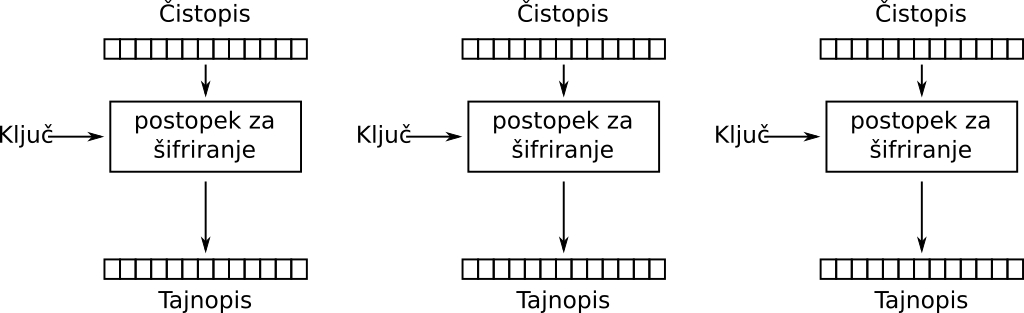
\includegraphics[width=\textwidth]{images/ECB_encryption}
    \caption{Šifriranje v načinu \gls{ECB}}
\label{fig:ecbenc}
\end{figure}

\begin{figure}[ht!]
  \centering
    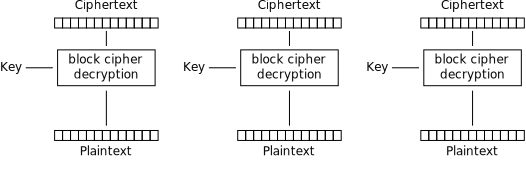
\includegraphics[width=\textwidth]{images/ECB_decryption}
    \caption{Dešifriranje v načinu \gls{ECB}}
\label{fig:ecbdec}
\end{figure}


Vse to so sicer dobrodošle lastnosti, vendar ima \gls{ECB} nekaj resnih pomanjkljivosti, zaradi katerih ni primeren za uporabo v resničnem svetu, ampak služi bolj kot opomin, da močni šifrirni algoritmi kot je \gls{AES}, ne zagotavljajo varnosti, če so uporabljeni na napačen način.

Slika~\ref{fig:ecbbad} prikazuje uporabo 128 bitne AES šifre v načinu ECB.\@ Na šifrirani sliki je še vedno možno razpoznati logotip Fakultete za računalništvo in informatiko, kar pomeni da tak način šifriranja ne zagotavlja varnosti.

\begin{figure}[ht!]
  \centering
  \begin{subfigure}[b]{0.3\textwidth}
    
\includegraphics[width=\textwidth]{images/LogoFRI}
    \caption{Original}
\label{fig:logoFRIorig}
  \end{subfigure}
  \begin{subfigure}[b]{0.3\textwidth}
    
\includegraphics[width=\textwidth]{images/LogoFRI_ecb}
    \caption{AES-128-ECB}
\label{fig:logoFRIECB}
  \end{subfigure}
  \begin{subfigure}[b]{0.3\textwidth}
    
\includegraphics[width=\textwidth]{images/LogoFRI_cbc}
    \caption{AES-128-CBC}
\label{fig:logoFRICBC}
  \end{subfigure}
  \caption{Primer različnih načinov šifriranja, uporabljenih na logotipu FRI}
\label{fig:ecbbad}
\end{figure}

\subsubsection{CBC}
\label{subs:CBC}

V načinu \Gls{CBC} se vsak blok čistopisa pred šifriranjem z operacijo $XOR$ zmeša z tajnopisom prejšnjega bloka. Tak pristop naredi vsak naslednji blok odvisen od vseh prejšnjih blokov. S tem se rešimo problema ponavljajočih se vzorcev v tajnopisu, kot smo jih videli v načinu \acrshort{ECB} (slika~\ref{fig:ecbbad}). Posebni primer je prvi blok, saj tu nimamo na voljo tajnopisa prejšnjega bloka, s katerim bi izvedli operacijo $XOR$, zato namesto tajnopisa prejšnjega bloka uporabimo \acrfull{IV}. Dodatno nam naključni \gls{IV} doda tudi element naključnosti v tajnopis, kar pomeni, da tudi, če šifriramo enako sporočilo z enakim ključem, tajnopis ne bo enak, saj smo uporabili drugačen \gls{IV}.

Slabost takega pristopa pa je, da je operacija šifriranja strogo zaporedna, saj naslednjega bloka ne moremo šifrirati, dokler ne končamo šifriranja trenutnega bloka.

\begin{figure}[ht!]
  \centering
    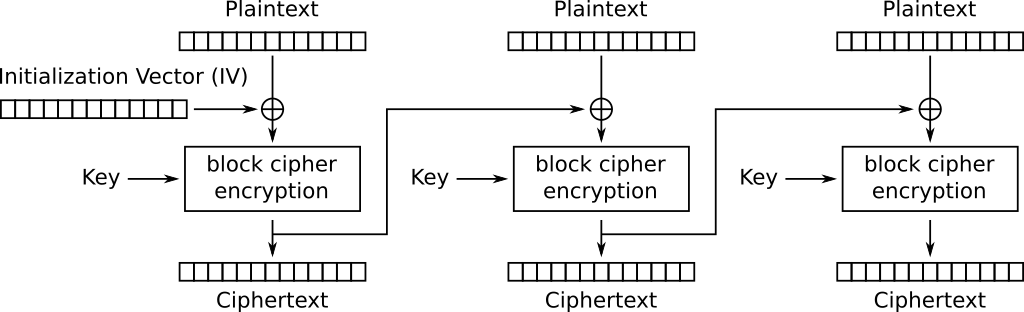
\includegraphics[width=\textwidth]{images/CBC_encryption}
    \caption{Šifriranje v načinu \gls{CBC}}
\label{fig:cbcenc}
\end{figure}

\begin{figure}[ht!]
  \centering
    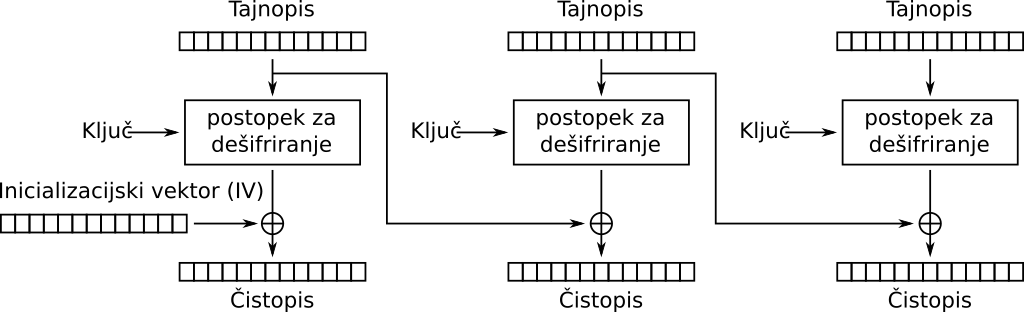
\includegraphics[width=\textwidth]{images/CBC_decryption}
    \caption{Dešifriranje v načinu \gls{CBC}}
\label{fig:cbcdec}
\end{figure}

\subsubsection{CFB}
\label{subs:CFB}

V \gls{CFB} načinu delovanja se bločna šifra uporablja kot tokovna. Prednost takega načina delovanja je, da ni potrebe po dopolnjevanju sporočila, prav tako pa se uporablja samo ena smer delovanja bločne šifre (to je ponavadi smer šifriranja), kar poenostavi implementacijo takega načina v strojni opremi.

Kot se vidi na slikah~\ref{fig:cfbenc} in~\ref{fig:cfbdec}, se v tem načinu delovanja bločna šifra uporablja le za generiranje naključnega zaporedja, tajnopis pa je rezultat operacije $XOR$ med čistopisom in naključnim zaporedjem, podobno kot pri enkratnem ščitu (angl.\ one time pad).

\begin{figure}[ht!]
  \centering
    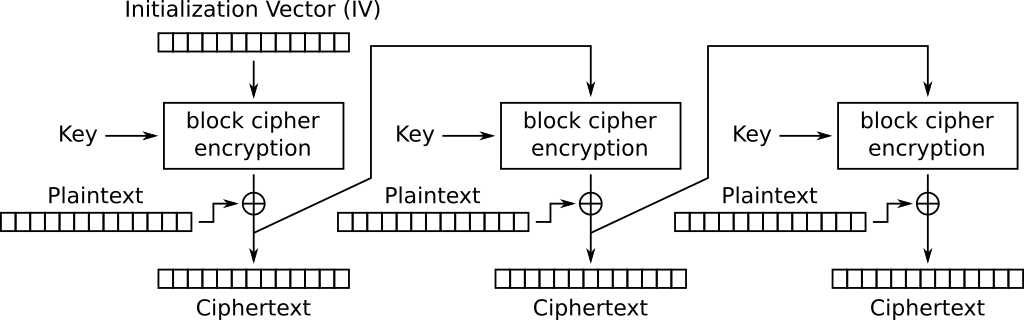
\includegraphics[width=\textwidth]{images/CFB_encryption}
    \caption{Šifriranje v načinu CFB}
\label{fig:cfbenc}
\end{figure}

\begin{figure}[ht!]
  \centering
    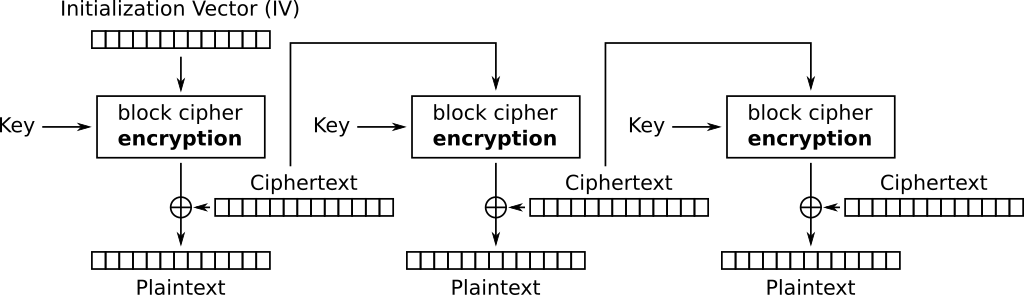
\includegraphics[width=\textwidth]{images/CFB_decryption}
    \caption{Dešifriranje v načinu CFB}
\label{fig:cfbdec}
\end{figure}

\subsubsection{OFB}
\label{subs:OFB}

\gls{OFB} je podoben načinu \gls{CFB}, s to razliko, da se za ustvarjanje naključnega zaporedja uporablja samo \gls{IV}. V primeru, da šifriramo daljša sporočila, je to lahko problematično, saj lahko pride do cikla v naključnem zaporedju. To se zgodi v primeru, da se v naključnem zaporedju pojavi blok, katerega tajnopis je enak IV.\@

\begin{figure}[ht!]
  \centering
    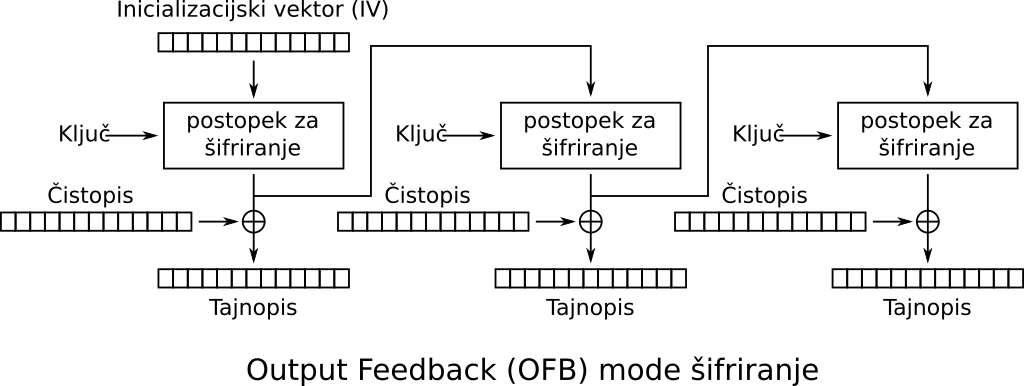
\includegraphics[width=\textwidth]{images/OFB_encryption}
    \caption{Šifriranje v načinu OFB}
\label{fig:ofbenc}
\end{figure}

\begin{figure}[ht!]
  \centering
    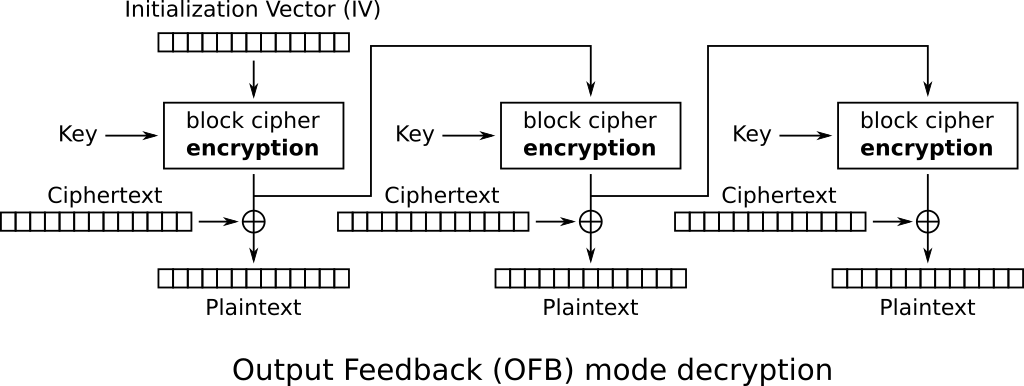
\includegraphics[width=\textwidth]{images/OFB_decryption}
    \caption{Dešifriranje v načinu OFB}
\label{fig:ofbdec}
\end{figure}

\section{Asimetrični kriptosistemi}
\label{sec:Asimetrični kriptosistemi}

Eden večjih problemov simetričnih šifrirnih algoritmov je distribucija ključev. V kolikor želita dve osebi svojo komunikacijo zaščititi z uporabo simetričnega šifrirnega algoritma, si morata najprej izmenjati ključ. Dobra praksa je tudi, da se izognemo ponovni uporabi istega ključa, kar v praksi pomeni, da si moramo z vsako osebo, s katero želimo komunicirati izmenjati ključ in hitro se izkaže, da omrežje $n$ ljudi potrebuje $\frac{n(n-1)}{2}$ ključev. Če to preslikamo na omrežje kot je internet, ki ga uporablja približno 40 odstotkov svetovne populacije. Vzemimo pesimistično oceno, da si vsak uporabnik interneta lasti samo eno elektronsko napravo, ki uporablja varno komunikacijo in tako omrežje potrebuje $\approx 4*10^{18}$ izmenjav ključa.

Rešitev za ta problem so lahko asimetrični kriptosistemi, oziroma kriptografija javnih ključev. Taki sistemi ne uporabljajo samo enega, ampak dva ključa. Javni ključ poznajo vsi in ga uporabijo za šifriranje sporočil. Sporočila, šifrirana z javnim ključem, lahko dešifrira samo imetnik zasebnega ključa.

Asimetrični kriptosistemi slonijo na predpostavki, da so nekateri matematični v eno smer preprosto izračunljivi, v drugo pa preprosto pretežki, da bi jih bilo možno rešiti v razumnem časovnem okvirju. Eden takih problemov je faktorizacija števil. Če si izmislite dve dokaj veliki praštevili $p$ in $q$, ju med seboj pomnožite, dobite novo število $n$, za katero ni tako preprosto ugotoviti iz katerih faktorjev je sestavljeno, ob predpostavki, da ne poznamo $p$ in $q$.

Na žalost so asimetrični kriptosistemi, tudi zaradi svojega ozadja v netrivialnih matematičnih problemih, veliko počasnejši od simetričnih. V praksi se zato pogosto uporablja kombinacija obeh tipov sistemov. V prvi fazi se za dogovor o ključu uporabi asimetrični kriptosistem, ko pa se obe strani dogovorita o skupnem ključu, pa preklopita na simetrični kriptosistem.

\subsection{Dogovor o ključu Diffe-Hellman}
\label{sub:Dogovor o kljucu Diffe-Hellman}

Dogovor o ključu Diffe-Hellman je bil prvi javno objavljen algoritem, ki uporablja princip javnih in zasebnih ključev. V praksi omogoča, da se dva neznanca preko nezavarovanega kanala kot je internet dogovorita za skupni ključ, ki ga bosta uporabljala za nadaljnjo komunikacijo. Prva sta ga objavila W. Diffie in M. Hellman leta 1976~\cite{diffie1976new}, vendar se je kasneje izkazalo, da je angleška tajna služba odkrila princip kriptografije javnih ključev že leto poprej, a je to ostalo tajno do leta 1997.

Metoda temelji na reševanju problema diskretnega logaritma, za katerega matematiki verjamejo, da ne obstaja algoritem, ki ga bi bil sposoben rešiti v sprejemljivih časovnih okvirjih (izjema so algoritmi, ki tečejo na kvantnih računalnikih, vendar je to povsem drug svet).

Originalna različica algoritma uporablja multiplikativno grupo števil po modulu $p$, kjer je $p$ praštevilo in $g$ primitivni koren števila $p$.

Recimo, da se želita Anita in Bojan preko interneta dogovoriti o skupnem ključu, ki ga bosta uporabljala za nadaljnjo komunikacijo. To lahko storita po postopku, ki je opisan v definiciji~\ref{def:dhprob}.

\begin{mdframed}[frametitle={Izmenjava ključa Diffe-Hellman}]
\begin{minipage}{\textwidth}
\begin{defn}

\begin{enumerate}
	\item Anita in Bojan se dogovorita o skupnih parametrih, ki jih bosta uporabljala v algoritmu. To je praštevilo $p$ in primitivni koren praštevila~$g$.
	\item Anita si izbere skrivno število $a$, izračuna $A=g^a \mod p$ in pošlje $A$ Bojanu.
	\item Bojan si izbere skrivno število $b$, izračuna $B=g^b \mod p$ in pošlje $B$ Aniti.
	\item Anita izračuna $s=B^a \mod p$.
	\item Bojan izračuna $s=A^b \mod p$.
	\item Anita in Bojan sta dobila enak rezultat $s$, ki ga sedaj lahko uporabita kot skupni ključ za nadaljnjo komunikacijo.
\end{enumerate}

\vspace{0.5cm}

Oba sta izračunala enak rezultat, ker velja:
$$
A^b \equiv g^{ab} \equiv g^{ba} \equiv B^a \mod p
$$
\label{def:dhprob}
\end{defn}
\end{minipage}
\end{mdframed}


\subsection{RSA}
\label{sub:RSA}

Medtem, ko prej opisana metoda omogoča samo dogovor o skupnem ključu, pa je bil \gls{RSA} prvi pravi kriptosistem, ki je uporabljal javne ključe. Varnost \gls{RSA} temelji na tem, da je faktorizacija produkta dveh velikih praštevil težko rešljiv problem za današnje računalnike.

\begin{mdframed}[frametitle={RSA kriptosistem}]
\begin{minipage}{\textwidth}
  \begin{defn}
    Javni ključ je par $(n, e)$, zasebni ključ pa par $(n, d)$, ki ju dobimo po naslednjem postopku:

    \begin{enumerate}
    \item Izberemo dve naključni, približno enako veliki praštevili $p$ in $q$
    \item Izračunamo modul $n=pq$
    \item Izračunamo $\varphi(n)=\varphi(p)\varphi(q)=(p-1)(q-1)$
    \item Izberemo število $e$, tako da $1<e<\varphi(n)$ tako da je $e$ tuje $\varphi(n)$
    \item Izračunamo $d$, tako da $d \equiv e^{-1} \pmod{\varphi(n)}$
    \end{enumerate}

    Poleg zasebnega ključa moramo moramo paziti tudi na zasebnost vrednosti $p$, $q$ in $\varphi(n)$.

    Sporočilo $m \in \mathbb{Z}$ šifriramo po naslednjem postopku: $$c=e(m)=m^e \mod n$$

    Dešifriranje je podobna operacija, le da za eksponent vzamemo zasebni ključ: $$m=d(c)=c^d \mod n$$
    \label{def:rsa}
  \end{defn}
\end{minipage}
\end{mdframed}

Definicija~\ref{def:rsa} ponazori osnovno idejo kriptosistema RSA, vendar je potrebno še nekaj korakov, da jo dopolnimo do varnega kriptosistema. Eden od problemov, ki jih lahko hitro opazimo, da lahko napadalec iz tajnopisa $c = e(m)$, za poljuben $t$, izračuna tajnopis za sporočilo $mt$.
$$
e(m)*t^e \mod n = m^et^e \mod n = (mt)^e \mod n = e(mt)
$$

Tej lastnosti rečemo gnetljivost (angl.\ malleability), saj napadalec lahko samo s poznavanjem javnih parametrov kriptosistema in tajnopisa $c$, skonstruira nov tajnopis $c'$, ki se dešifrira v čistopis, ki je na nek način povezan s čistopisom, ki pripada $c$. V splošnem velja, da je to neželjena lastnost varnega kriptosistema, vendar bomo v poglavju \ref{sec:Homomorfni kriptosistemi} spoznali, da s tem, ko dovolimo gnetljivost kriptosistema, odpremo vrata popolnoma novim načinom uporabe kriptografije v oblaku.


\chapter{Uporaba kriptografije v oblaku}
\label{chap:Uporaba kriptografije v oblaku}

Največji problem uporabe šifriranja v oblaku je v bistvu enak kot povsod kjer poskušamo zagotoviti varnost na tak in drugačen način. Potrebno je najti kompromis med zadovoljivim nivojem varnosti in uporabnostjo. Trivialno je narediti 100\% varen sistem, vendar ta verjetno ne bo kaj prida uporaben.

Prav tako ločimo tri stanja digitalnih podatkov: podatki v mirovanju, podatki v gibanju in podatki v uporabi. V vsakem stanju obstajajo različne varnostne zahteve, zato se potrebni različni pristopi. Jaber in Zolkipli\cite{jaber2013use} sta uporabila tabelo~\ref{tbl:cloudtriad}, ki lepo ponazori načine uporabe kriptografije glede na različna stanja podatkov.

\begin{table}[ht!]
  \centering
  \begin{tabular}{lllll}
                                        & Podatki v mirovanju                   & Podatki v uporabi                    & Podatki v gibanju              &  \\ \cline{2-4}
    \multicolumn{1}{l|}{Zaupnost}       & \multicolumn{1}{l|}{Simetrični kriptosistemi} & \multicolumn{1}{l|}{Homomorfne šifre} & \multicolumn{1}{l|}{TLS}        &  \\ \cline{2-4}
    \multicolumn{1}{l|}{Istovetnost}    & \multicolumn{1}{l|}{MAC}              & \multicolumn{1}{l|}{Homomorfne šifre} & \multicolumn{1}{l|}{TLS}        &  \\ \cline{2-4}
    \multicolumn{1}{l|}{Razpoložljivost} & \multicolumn{1}{l|}{redundanca}       & \multicolumn{1}{l|}{redundanca}       & \multicolumn{1}{l|}{redundanca} &  \\ \cline{2-4}
  \end{tabular}
  \caption{Načini uporabe kriptografije v oblaku}
\label{tbl:cloudtriad}
\end{table}

Zgodovinsko gledano je bila kriptografija izumljena z motivom varovanja komunikacij, torej podatkov v gibanju, vendar na problem varovanja podatkov v mirovanju lahko gledamo kot na komunikacijo s samim sabo. To nam predvsem poenostavi problem distribucije ključev, zato so za varovanje podatkov v mirovanju zelo primerne simetrične šifre.

Na začetku obdobja računalništva se je največ pozornosti posvečalo predvsem varnosti podatkov v mirovanju, saj so se informacijski sistemi nahajali znotraj podjetja, oziroma so bili do podjetja povezani preko najetih vodov. Prav tako so se podatki obdelovali na strojni opremi, ki je bila v lasti podjetja in se je nahajala na varni lokaciji. S prihodom storitev v oblaku, se je ta paradigma spremenila. Podatke je treba najprej prenesti v oblačni sistem, največkrat kar preko interneta. Prav tako podatke v oblak pošljemo z namenom, da jih bomo tam obdelovali in analizirali, kar pomeni da je potrebno poskrbeti tudi za varnost podatkov v uporabi.

To se odraža tudi v pristopih k varovanju podatkov v različnih stanjih. Dočim za varovanje podatkov v mirovanju obstajajo ustaljene prakse, pa za ostali dve področji velja, da se nenehno spreminjata. Na področju varovanja podatkov v gibanju, ki ga v primeru oblačnih sistemov večinoma pokrivata kriptografska protokola \acrfull{SSL} in njegov naslednik \acrfull{TLS}, je v zadnjih letih prišlo do odkritji različnih napadov in posledično opustitve določenih verzij protokolov, ker te niso več zagotavljale zadovoljivega nivoja varnosti. Drugačna pa je situacija na področju varovanja podatkov v uporabi, saj v preteklosti ni bilo velike potrebe po praktični implementaciji takih kriptografskih protokolov, vendar se je s prihodom oblačnih storitev tudi to področje začelo pospešeno razvijati.

\section{Funkcionalni kriptosistemi}
\label{sec:Funkcionalni kriptosistemi}

Pred iznajdbo asimetričnih šifrirnih shem, je veljalo prepričanje, da če želimo vzpostaviti šifrirano komunikacijo, si morata najprej obe strani izmenjati skrivni ključ. V sedemdesetih letih sta Diffe in Hellman~\cite{diffie1976new} to prepričanje postavila na glavo in predstavila algoritem za izmenjavo ključa, kjer ni potrebe po varnem kanalu.
Podobno je še do pred kratkim veljalo prepričanje: \textit{(1) Šifrirano sporočilo je mogoče poslati samo eni osebi (prejemniku), ki si lasti pripadajoč dešifrirni ključ.} in  \textit{(2) Dešifriranje je možno samo na principu vse ali nič. Torej ali je prejemnik sposoben dešifrirati sporočilo v celoti (poseduje dešifrirni ključ), ali pa ga sploh ne more dešifrirati.}

To lahko predstavlja nekaj nevšečnosti v oblačnih sistemih, kjer želimo uporabiti šifriranje. V primeru, da želimo deliti šifrirane datoteke, je potrebno za vsakega uporabnika ustvariti unikaten ključ in na novo šifrirati datoteko. V praksi se je sicer možno izogniti vsakokratnemu šifriranju, vendar bi bila veliko lepša rešitev, če bi lahko datoteko šifrirali tako, da jo lahko dešifrira več uporabnikov. Podoben primer so strežniški dnevniki in revizijske sledi, ki lahko vsebujejo občutljive podatke o uporabnikovi aktivnosti ob določenem času. Da uporabnikom zagotovimo visoko stopnjo zasebnosti, lahko take datoteke šifriramo. Vendar se pojavi problem, če policija po nalogu sodišča od ponudnika zahteva strežniške dnevnike skupaj z dešifrirnim ključem. Če je dešifriranje možno samo na principu vse ali nič, policija pridobi vpogled v aktivnost vseh uporabnikov sistema, ne le osumljenca. Rešitev bi bila, da za vsakega uporabnika izberemo unikaten ključ, vendar če želimo policiji omejiti tudi obdobje, za katerega lahko dešifrira podatke, je potrebno ta ključ rotirati in število teh ključev lahko naraste čez vse razumne meje. Priročnejša rešitev bi bila, če bi lahko uporabili tako šifrirno shemo, kjer lahko ključ dešifrira le del tajnopisa.

Izkaže se, da take šifrirne sheme res obstajajo, vendar je to področje kriptografije še dokaj novo in obstaja še veliko odprtih problemov. Čeprav so bili mnogi algoritmi, ki jih sedaj uvrščamo v to kategorijo odkriti že prej, pa je bila prva formalizacija javno predstavljena šele leta 2011. V nadaljevanju bomo na kratko povzeli definicijo, kot je bila predstavljena v članku D. Boneh in drugih~\cite{boneh2011functional}.

\begin{mdframed}[frametitle={Funkcionalnost}]
\begin{defn}
Funkcionalnost $F$, definirana na $(K, X)$ je funkcija $$F: K \times X \rightarrow {\{}0,1{\}}^*$$ predstavljena kot determinističen Turingov stroj. Množica $K$ je prostor vseh ključev in množica $X$ je prostor vseh čistopisov. Zahtevamo tudi, da množica $K$ vsebuje prazen ključ $\epsilon$.
\label{def:functionality}
\end{defn}
\end{mdframed}


\begin{mdframed}[frametitle={Funkcionalni kriptosistem}]
\begin{defn}
Funkcionalni kriptosistem za funkcionalnost~$F: K \times X \rightarrow {\{}0,1{\}}^*$ je četvorka algoritmov:
\begin{align*}
  (pp, mk) \leftarrow setup(1^\lambda) \\
  sk \leftarrow keygen(mk, k) \\
  c \leftarrow enc(pp, x)  \\
  y \leftarrow dec(sk, c)  \\
\end{align*}
kjer zahtevamo, da velja: $y=F(k, x)$.
\textit{Setup} predstavlja postopek za generiranje javnega ($pk$) in glavnega zasebnega ključa ($mk$), $\lambda$ pa je varnostni parameter. Postopek \textit{kygen} iz glavnega zasebnega ključa $mk$ in ključa $k$ ustvari skrivni ključ $sk$. Postopek \textit{enc} je šifrirni postopek, ki sporočilo $x$ šifrira z javnim ključem $pp$. Dešifriranje je postopek \textit{dec}, ki kot vhod vzame skrivni ključ $sk$ in tajnopis $c$, kot rezultat pa vrne $y$, ki je pravzaprav rezultat funkcionalnosti $F$.
\label{def:fe}
\end{defn}
\end{mdframed}

V funkcionalni šifrirni shemi za funkcionalnost~$F(\cdot, \cdot)$ lahko \gls{authority}, ki si lasti glavni skrivni ključ, ustvari ključ~$sk_k$, s katerim uporabnik izračuna vrednost funkcije~$F(k, x)$ iz tajnopisa za~$x$. Recimo, da je možno, da za $F$ vzamemo katerokoli funkcijo, ki jo je možno opisati z determinističnim turingovim strojem. To nam odpre možnost, da v šifrirno shemo vgradimo ``program'' za nadzor dostopa in s tem zaobidemo omejitve, omenjene v prvem odstavku.

Izkaže se, da je možno tudi povsem klasične asimetrične šifrirne sheme predstaviti v obliki funkcionalne šifrirne sheme, vendar so veliko bolj zanimive sheme, ki za ključe uporabljajo kar uporabnikovo identiteto - \gls{IBE} in njihova nadgradnja, ki je predstavljena v naslednjem poglavju.

\subsection{Šifriranje na osnovi atributov in predikatov}
\label{sub:Šifriranje na osnovi atributov in predikatov}

Šifriranje na osnovi atributov in predikatov je poseben primer funkcionalne šifrirne sheme z vgrajeno kontrolo dostopa. Za začetek si poglejmo naslednji primer:

Anita ima datoteko $X$, ki bi jo rada delila s skupinama \textbf{Prijatelji} in \textbf{Znanci}. Prav tako ima datoteko $Y$, ki bi jo rada delila s skupinama \textbf{Družina} in \textbf{Prijatelji}. To lahko stori tako, da ustvari en ključ za datoteko $X$ in ta ključ deli s \textbf{Prijatelji} in  \textbf{Znanci}, nato ustvari drug ključ za datoteko $Y$ in ta ključ deli s skupinama \textbf{Družina} in \textbf{Prijatelji}. Problem je, da mora Anita za vsako datoteko, ki jo želi deliti, ustvariti nov ključ.

Naivna rešitev tega problema bi bila, da Anita ustvari en ključ za vsako skupino ljudi, s katerimi želi deliti datoteke. Vendar življenje ni preprosto, in lahko se zgodi, da neka oseba pripada večim skupinam s katerimi želi Anita deliti datoteke. Prav tako si lahko zaželi deliti neko datoteko samo z ljudmi, ki so hkrati \textbf{Prijatelji} in \textbf{Sodelavci}. Recimo, da je to datoteka $Z$. Tako datoteko lahko najprej šifrira s ključem, ki pripada skupini \textbf{Prijatelji}, in nato še s ključem, ki pripada skupini \textbf{Sodelavci}. Naivno bi mislili, da je to dobra rešitev, vendar se izkaže, da tak sistem ni odporen proti zaroti. Šifrirano datoteko lahko kot posamezniki odprejo samo ljudje, ki pripadajo obema skupinama, saj imajo le oni v posesti oba ključa. Vendar pa se lahko proti Aniti zarotita dva posameznika, kjer noben od njiju ne pripada obema skupinama hkrati, vendar imata skupaj dostop do obeh ključev, saj vsak od njiju pripada eni od skupin.

Možnost dešifriranja določajo pravila, ki so predstavljena z drevesi, kjer so notranja vozlišča logične operacije, listi pa predikati, ki so lahko zadovoljeni ali nezadovoljeni. Drevo beremo od listov proti korenu in za vsako notranje vozlišče ugotovimo ali je v zadovoljenem ali nezadovoljenem stanju. Na koncu pridemo do korena drevesa, in dešifriranje uspe samo v primeru, da je koren drevesa v zadovoljenem stanju.

Poznamo dve vrsti šifriranja na osnovi parametrov. V prvem je drevo, ki določa pravila shranjeno v ključu  (angl. \acrlong{KP-ABE}), v drugem primeru pa je shranjeno v tajnopisu (angl. \acrlong{CP-ABE}).

\begin{mdframed}[frametitle={Funkcionalni kriptosistem s predikati}]
\begin{defn}
Velikokrat ima čistopis $x \in X$, določeno strukturo, recimo da je v obliki para $(\texttt{ind}, m) \in I \times M$, kjer imenujemo \texttt{ind} indeks in $m$ koristni tovor. Primer je lahko e-poštni sistem, kjer je indeks identiteta pošiljatelja, koristni tovor pa e-sporočilo.

Definirajmo predikat $P: K \times I \rightarrow {\{}0, 1{\}}$ in funcionalnost $F: K \times X \rightarrow X \cup \bot$:

\begin{gather*}
F(k, (\texttt{ind}, m)) = \begin{cases}
m & \text{če velja } P(k, \texttt{ind}) = 1\\
\bot & \text{če velja } P(k, \texttt{ind}) = 0\\
\end{cases}
\end{gather*}

Če tako funkcionalnost uporabimo v definiciji~\ref{def:fe}, to pomeni, da dešifrirni postopek $dec(sk, c)$, kjer je $sk$ skrivni ključ za $k$ in $c = enc(pp, (\texttt{ind}, m))$ tajnopis, vrne čistopis, če in samo če $P(k, \text{\texttt{ind}})=1$.

\label{def:fepredicate}
\end{defn}
\end{mdframed}

Funkcionalni kriptosistem s predikati, podan v definiciji~\ref{def:fepredicate}, lahko uporabimo za izgradnjo KP-ABE in CP-ABE kriptosistemov. Iz definicij~\ref{def:kpabe} in~\ref{def:cpabe} lahko vidimo da sta si sistema zelo podobna, razlika je le katere informacije hranimo v ključu $k$ in katere v funkcionalnosti $F$. V KP-ABE kriptosistemu nam ključ kodira formulo $\phi$ (pravilo) za dostop do podatkov, tajnopis pa vsebuje atribute, katerih vrednost je lahko \textit{DA} ali \textit{NE} (logična $1$ ali logična $0$). Dešifriranje v takem sistemu je uspešno le v primeru, da formula, podana v ključu, vrne rezultat 1 (\textit{DA}) za dane atribute $\vec{z}$ v tajnopisu. Kriptosistem CP-ABE, definiran v \ref{def:cpabe}, uporablja enak princip, le da so atributi kodirani v ključu, formula za dostop do podatkov pa v tajnopisu.

\begin{mdframed}[frametitle={KP-ABE kriptosistem}]
\begin{minipage}{\textwidth}
\begin{defn}
KP-ABE kriptosistem v $n$ spremenljivkah (atributih) je funkcionalni kriptosistem s predikatom iz definicije~\ref{def:fepredicate}, kjer:

\begin{enumerate}
  \item Prostor ključev $K$ je množica logčnih (Boolovih) formul $\phi$ v n spremenljivkah $\vec{z} = (z_1, \ldots, z_n)$. Naj $\phi(\vec{z})$ označuje vrednost formule $\phi$ za $\vec{z}$.
  \item Čistopis je par $(\texttt{ind} = \vec{z}, m)$, kjer je indeksni prostor $I: {\{}0,1{\}}^n$.
  \item Predikat $P: K \times I \rightarrow {\{}0, 1{\}}$ definiramo kot:
  \begin{gather*}
  P(\phi \in K \setminus {\{}\epsilon{\}}, \texttt{ind} = \vec{z} \in I) = \phi(\vec{z})
  \end{gather*}
\end{enumerate}
\label{def:kpabe}
\end{defn}
\end{minipage}
\end{mdframed}

\begin{mdframed}[frametitle={CP-ABE kriptosistem}]
\begin{minipage}{\textwidth}
\begin{defn}
CP-ABE kriptosistem v $n$ spremenljivkah (atributih) je funkcionalni kriptosistem s predikatom iz definicije~\ref{def:fepredicate}, kjer:

\begin{enumerate}
  \item Prostor ključev $K := {\{}0,1{\}}^n$ je množica vseh vektorjev $\vec{z}$, ki predstavljajo točke, v katerih lahko izračunamo vrednost formule $\phi$.
  \item Čistopis je par $(\texttt{ind} = \phi, m)$, kjer je indeksni prostor $I$ možica vseh logičnih formul v $n$ spremenljivkah.
  \item Predikat $P: K \times I \rightarrow {\{}0, 1{\}}$ definiramo kot:
  \begin{gather*}
  P(\vec{z} \in K \setminus {\{}\epsilon{\}}, \texttt{ind} = \phi \in I) = \phi(\vec{z})
  \end{gather*}
\end{enumerate}
\label{def:cpabe}
\end{defn}
\end{minipage}
\end{mdframed}


\section{Homomorfni kriptosistemi}
\label{sec:Homomorfni kriptosistemi}

Homomorfizem je lastnost, da je določena algebraična operacija nad dvema čistopisoma ekvivalentna neki drugi operaciji nad pripadajočima tajnopisoma. To pomeni, da namesto, da naredimo neko operacijo nad čistopisom, lahko izvedemo homomorfno operacijo nad tajnopisom in končni rezultat bo isti. Take kriptosistemi bi v teoriji lahko omogočili varno računanje v oblaku, saj je možno vse operacije izvajati nad tajnopisi, tako da ni potrebe, da oblačni sistem kadarkoli pride v stik s čistopisom podatkov.

Potrebna lastnost homomorfne šifre je \glslink{malleable}{gnetljivost} (angl.\ malleability), ki je sicer v večini ostalih shem nezaželena lastnost. Gnetljivost omogoča spremembo tajnopisa na tak način, da se ta dešifrira v čistopis, ki je na nek način povezan z originalnim čistopisom. Če imamo dan tajnopis za $m$, to pomeni, da je možno izračunati nov tajnopis, ki se bo dešifriral v vrednost $f(m)$ za neko funkcijo $f$, brez da bi sploh vedeli vrednost $m$.

Ločimo dva tipa homomorfnih šifer, glede na to, katere operacije lahko opravimo nad tajnopisi. V prvo skupino spadajo delno homomorfni sistemi, kot so RSA brez dopolnjevanja, ElGamal in drugi. Taki sistemi so homomorfni samo za eno operacijo in kot taki ne prav zanimivi za splošno uporabo, je pa z njimi možno implementirati rešitev kot so recimo varne e-volitve. Veliko bolj zanimivi pa so popolnoma homomorfni sistemi, kjer je nad tajnopisi možno izvesti poljubno operacijo. Prvi popolnoma homomorfni kriptosistem je v svoji doktorski disertaciji predstavil C. Gentry~\cite{gentry2009fully}, vendar se njegova implementacija ni izkazala za najbolj praktično. Prvi problem predstavlja velikost javnega ključa, ki sega od 70 MB do 2,3 GB, odvisno od stopnje varnosti, ki jo želimo. Prav tako je problematična hitrost take sheme, saj obdelava enega bita informacije traja nekje med 30 sekundami in 30 minutami.

Za občutek lahko predstavimo nekoliko homomorfno šifrirno shemo, ki je bila predstavljena v~\cite{gentry2010computing}. Shema je veliko preprostejša od prve sheme v doktorski disertaciji C. Gentry-a, saj uporablja preprosto številsko aritmetiko, vendar ima problem, da omogoča samo omejeno število evalvacij funkcije, preden rezultat postane neuporaben.

\begin{description}
  \item[KeyGen]: za ključ izberemo naključno liho P-bitno celo število
  \item[$e_k(m)$]: Šifriranje $m \in \{0,1\}$ poteka tako, da najprej izberemo naključno N-bitno število $m'$, da velja $m' = m \mod 2$. Tajnopis je $c=m'+pq$, kjer je $q$ naključno $Q$-bitno celo število.
  \item[$d_k(m)$]: Rezultat dešifriranja je $(c \mod p) \mod 2$, kjer velja $c'=c \mod p$ in $-p/2 < c' < p/2$ in $p$ deli $c-c'$.
\end{description}

V taki shemi je možno tajnopise seštevati, odštevati in množiti po modulu 2. Ker seštevanje in množenje po modulu 2 hkrati predstavlja tudi logična vrata $AND$ in $XOR$, lahko v takem sistemu ovrednotimo poljubno funkcijo, ki jo je možno predstaviti digitalno vezje. Problem nastane, ker vsaka od teh operacij poveča količino ``šuma'', ki smo ga dodali pri šifriranju, in če ta naraste preko neke meje, sporočila ni več možno dešifrirati.\todo{napisi se vec}

Problem šuma je mogoče rešiti tako, da podatke dešifriramo. Če nam uspe dešifrirno funkcijo predstaviti kot logično vezje, ki ga je možno ovrednotiti v dani shemi, smo na dobri poti da zmanjšamo šum. Kriptosistemom, ki so sposobni te operacije rečemo, da so \glslink{bootstrappable}{\textit{samozagonski}} (angl.\ bootstrappable), in možno je pokazati, da iz takega sistema lahko sestavimo popolnoma homomorfen kriptosistem. Kljub temu, da ta postopek omogoča, da pridemo do popolnoma homomorfnega kriptosistema, pa je daleč od idealnega. Ovrednotenje dešifrirne funkcije, predstavljene kot digitalno vezje je računsko zahteven postopek, prav tako pa tajnopis enega samega bita informacije zasede precej več prostora kot pripadajoč čistopis. Zato se v zadnjem času veliko raziskav usmerja v kriptosisteme, kjer \textit{bootstraping} ni potreben.\todo{Learning with errors}


\section{Varovanje podatkov v mirovanju}
\label{sec:Varovanje podatkov v mirovanju}

Podatke v mirovanju predstavljajo vsi podatki na trajnem pomnilniku, izključujoč podatke, ki so trenutno v gibanju in podatke, ki so trenutno v delovnem pomnilniku računalnika. Praviloma so to podatki, ki se ne spreminjajo pogosto, oziroma arhivski podatki, ki se sploh ne spreminjajo. Količinsko predstavljajo glavnino vseh podatkov, kar pomeni, da morajo biti kriptografski algoritmi, ki delujejo na teh podatki hitri. Zato so za varovanje takih podatkov zelo primerni simetrični kriptosistemi.

Podatki v mirovanju so dolgotrajne narave, kar pomeni da je dolgotrajna tudi skrb za varnost šifrirnih ključev, ki nam zagotavljajo dostop do teh podatkov. V preteklosti so bili ključi ``shranjeni'' kar v uporabnikovi glavi, vendar je ob količini podatkov s katerimi operiramo danes, to žal postala misija nemogoče. Dodaten problem predstavlja dejstvo, da je do podatkov pogosto potreben povsem avtomatski dostop, brez posredovanja človeka.

V kontekstu oblačnih sistemov je pri zagotavljanju varnosti podatkov v mirovanju najbolj problematičen del prav upravljanje s ključi, saj je potrebno poskrbeti za ključe velikega števila uporabnikov. Prav tako je s stališča varnosti neodgovorno, da ustvarjanje in upravljanje šifrirnih ključev zaupamo tretji osebi (ponudniku storitve). Zato je v primeru, da je potrebno zagotoviti visoko stopnjo varnosti, kljub temu pa želimo podatke hraniti v oblaku, najbolj primerno šifriranje podatkov še preden jih pošljemo v oblak, tako imenovano \textit{client-side} šifriranje. Prednosti so očitne, saj šifrirni ključ nikoli ne zapusti našega računalnika, tako da smo lahko prepričani, da do naših podatkov ne more dostopati nihče.

Kot smo že omenili, so za šifriranje takih podatkov najprimernejše simetrične šifre. Predvsem se priporoča uporaba modernih kriptosistemov, ki poleg zasebnosti zagotavljajo tudi istovetnost podatkov. Primeri takih sistemov so \textit{Salsa20-Poly1305}, \textit{Chacha20-Poly1305} in \textit{AES-GCM}. \textit{Salsa20}~\cite{bernstein2008salsa20} in \textit{Chacha20}~\cite{bernstein2008chacha} sta si si zelo podobni tokovni šifri (razlikujeta se le v krožni funkciji). Na drugi strani pa je bločna šifra \textit{AES} v načinu delovanja \textit{GCM}. \textit{AES} je industrijski standard za šifriranje podatkov, kar se pozna tudi v dobri strojni podpori za pohitritev šifriranja. Večina sodobnih procesorjev na arhitekturi \textit{x86} podpira nabor ukazov \textit{AES-NI}, ki znatno pohitrijo postopke šifriranja, kot je razvidno v tabeli~\ref{symmspeed}.

\begin{table}[]
\centering
\begin{tabular}{|l|l|}
\hline
                  & hitrost (GB/s) \\ \hline
AES-128-GCM       & 1,09           \\ \hline
CHACHA20-POLY1305 & 0,34           \\ \hline
CHACHA20-POLY1305 & 0,23           \\ \hline
\end{tabular}
\caption{Primerjava hitrosti treh priporočenih algoritmov. Test je bil izveden na procesorju Intel Core i5-2430M, ki podpira strojno pospešen AES}
\label{symmspeed}
\end{table}

Pri uporabi bločnih v kombinaciji z načinom delovanja (kar velja v $99\%$ primerov) se je potrebno zavedati, posledic rojstnodnevnega paradoksa~\cite{wiki:bdayparadox}. Glede na velikost bloka, obstaja zgornja meja za količino podatkov, ki jih je še varno šifrirati z istim ključem. V kolikor to mejo presežemo, obstaja možnost, da napadalcu s pomočjo rojstnodnevnega napada uspe dešifrirati delčke tajnopisa. Problem je še posebej pereč pri bločnih šifrah, ki uporabljajo 64 bitne bloke, saj je v tem primeru zgornja meja 32 GB, kar je v današnjih časih vse prej kot nedosegljiva količina podatkov. V primeru uporabe šifre z 128 bitnim blokom, se ta meja dvigne na 256 EB. Za šifro, ki uporablja n-bitne bloke, pa velja da je z njo varno šifrirati do $n*2^{n/2}$ bitov.


\begin{mdframed}[frametitle={Rojstnodnevni napad na način delovanja CBC}]
\begin{minipage}{\textwidth}
  \begin{defn}
    V načinu delovanja CBC šifriranje poteka tako: $$c_i = e_k(m_i \oplus c_{i-1})$$ kjer za $c_{-1}$ uporabimo \gls{IV}.

    Po tem isti ključ uporabimo za šifriranje več kot $2^{n/2}$ blokov, kjer je $n$ velikost bloka v bitih, obstaja velika verjetnost da pride do trka. Trk je dogodek, kjer napadalec v tajnopisu opazi dva enaka bloka ($c_i = c_j$). Ker šifrirna funkcija $e_k$ izvede samo permutacijo nad vhodnimi, lahko sklepamo, da je bil vhodni podatek $e_k$ za oba bloka enak ($m_i \oplus c_{i-1} = m_j \oplus c_{j-1}$). Iz tega sledi: $$m_i \oplus m_j = c_{i-1} \oplus c_{j-1}$$

    Napadalcu sta že znana oba tajnopisa $c_{i-1}$ in $c_{j-1}$, zato lahko ugane bodisi vrednost $m_j$, bodisi vrednost $m_i$ in preko zgornje formule izračuna manjkajočo vrednost ter tako dešifrira delček sporočila.
    \label{def:bdayattack}
  \end{defn}
\end{minipage}
\end{mdframed}


\subsection{Konvergentne šifrirne sheme}
\label{sub:Konvergentne šifrirne sheme}

V primeru oblačnih storitev, ki ponujajo hrambo podatkov v oblaku, pa je zaželena tudi sposobnost \glslink{deduplication}{izločanja dvojnikov (angl.\ deduplication)}, saj ta ponudniku storitve omogoča prihranke pri količini pomnilnika, porabljenega za hrambo datotek. Izločanje dvojnikov lahko deluje na nivoju datoteke ali pa na nivoju blokov. Najpreprostejša implementacija je na nivoju datoteke. Ob nalaganju datoteke v sistem se preveri zgoščena vrednost (hash) te datoteke, in v kolikor sistem ugotovi, da je datoteka z enako zgoščeno vrednostjo že shranjena v sistemu, samo poveča vrednost števca, ki kaže koliko kopij te datoteke že obstaja. Z uporabo tega principa lahko v sistemu obstaja praktično neomejeno število kopij iste datoteke, brez potrebe po neomejenih pomnilniških kapacitetah. Naprednejši načini izločanja dvojnikov datoteko najprej razbijejo na bloke konstantne ali spremenljive dolžine, in nato uporabijo isti postopek na blokih datoteke. Tako je možno dosečti še večje prihranke prostora na diskih.

Problem pa nastane, ko želimo izločanje dvojnikov uporabiti skupaj s šifriranjem. Praviloma želimo, da tajnopis izda karseda malo informacij o čistopisu, kateremu pripada. V praksi to pomeni, da za dva tajnopisa ne moremo ugotoviti, ali pripadata istemu čistopisu (isti datoteki), saj se v postopku šifriranja pogosto doda nek naključni element (recimo \gls{IV} v poglavju~\ref{sec:Nacini delovanja}). Tak pristop sicer omogoča doseganje \textit{semantične varnosti}, vendar onemogoči znatne prihranke pomnilniškega prostora ob poskusu izločanja dvojnikov. V kolikor želimo imeti oboje, je potrebno znižati varnostne zahteve. Če teoretičnemu napadalcu dovolimo, da ugotovi, da dva tajnopisa pripadata istemu čistopisu (torej tak kriptosistem ni \textit{semantično varen}) je izločanje dvojnikov možno.

\begin{mdframed}[frametitle={Semantična varnost}]
Kriptosistem je semantično varen, če iz tajnopisa ni mogoče na praktičen način pridobiti nobene informacije o čistopisu.
\end{mdframed}

V principu je potrebno poskrbeti, da šifriranje enakega čistopisa vsakič da enak tajnopis. To pomeni, da moramo vsakič uporabiti enak šifrirni ključ in tudi \gls{IV}, v kolikor ga dani kriptosistem zahteva. Lahko bi za vse datoteke vseh uporabnikov uporabili isti ključ in isti \gls{IV}, vendar taka implementacija nebi zagotavljala prav visoke varnosti. V veliko primerih ima šifriranje različnih čistopisov z enakim ključem in IV katastrofalne posledice za varnost. To nam pridejo na pomoč konvergentne kriptografske sheme. Prva taka shemo je podjetje Stac, Inc.\ patentiralo že leta 1995, v zadnjih letih pa so predvsem zaradi vse večje uporabe oblačnih shramb podatkov te sheme deležne veliko pozornosti. Osnovna ideja sheme je, da se šifrirni ključ izračuna iz čistopisa. Ponavadi se izračuna zgoščena vrednost čistopisa s pomočjo enosmerne zgoščevalne funkcije, nato pa se iz te vrednosti na determinističen način ustvari šifrirni ključ. Ker je zgoščena vrednost dveh enakih datotek tudi enaka, in postopek za izračun ključa determinističen, smo tako dosegli cilj, da se dve isti datoteki vedno zašifrirata v isti tajnopis.

Vendar pa imajo zaradi znižanih varnostnih zahtev taki sistemi tudi svoje ranljivosti. Ker je postopek šifriranja determinističen, tako lahko napadalec, ki si lasti enako datoteko, ugotovi ali ima to datoteko tudi kateri drug uporabnik. Na prvi pogled to sicer sicer ne izgleda tako problematično, vendar je na tak način mogoče ugotoviti, ali je uporabnik v sistem naložil piratsko vsebino ali pa prepovedano literaturo. V praksi se velikokrat uporabi izločanje dvojnikov na nivoju blokov, kar pa omogoča se bolj zvito izvedbo napada. V kolikor obstajajo datoteke, katerih vsebina je pretežno statična (recimo bančni izpiski), bodo tudi tajnopisi teh blokov v veliki meri enaki. Če ima napadalec dostop do podobnega bančnega izpiska, je obstaja verjetnost da se tajnopis napadalčevega in žrtvinega dokumenta razlikujeta samo v parih blokih. Napadalec lahko uporabi surovo silo in ustvari vse možne bloke, nato pa s pomočjo prvega napada ugotovi, kateri bloki pripadajo dokumentu žrtve napada. Takim napadom se je možno izogniti z uporabo ustreznega nadzora dostopa, kot je recimo opisano v članku~\cite{keelveedhi2013dupless}.

\subsection{Šifriranje in deljenje podatkov}
\label{sub:Šifriranje in deljenje podatkov}


\section{Varovanje podatkov v gibanju}
\label{sec:Varovanje podatkov v gibanju}

Za podatke v gibanju veljajo vsi podatki, ki se preko interneta pretakajo od uporabnika proti oblaku in obratno. Poleg tega pa so podatki v gibanju tudi vsi podatki, ki se prenašajo med različnimi strežniki znotraj oblačnega sistema.

Omrežja, po katerih podatki potujejo, velikokrat uporabljajo dinamične usmerjevalne algoritme, zato ne moremo vnaprej vedeti, po kateri poti bodo podatki potovali. Podatki v gibanju na svoji poti potujejo skozi veliko omrežnih naprav, ki imajo vpogled v podatke, prav tako pa jim ne moremo zaupati. Dodatno nevarnost predstavlja še \gls{MITM}, kjer napadalec izkoristi dinamičnost omrežja in se vrine na pot podatkov med uporabnika in sistem.

Podatki so v gibanju praviloma malo časa, zato ni potrebe po kompleksnem upravljanju ključev. S pomočjo algoritmov za varno izmenjavo ključev, kot je algoritem  Diffe-Hellman, opisan v poglavju~\ref{sub:Dogovor o kljucu Diffe-Hellman}, je možno, da se za vsako sejo uporabi nov, naključno generiran ključ.

Najbolj razširjen protokol za zaščito podatkov med tem ko so v gibanju je \gls{SSL} in njegov naslednik \gls{TLS}, pogosto imenovana s skupnim imenovalcem SSL/TLS. Poleg njega se predvsem za statične povezave med dvema omrežjema uporabljajo še protokoli iz družine VPN. Znotraj omrežja ponudnika pa se lahko uporabijo tudi tehnologije kot je VLAN. VLAN ne zagotavlja varnosti s pomočjo šifriranja, ampak deluje na principu omejevanja dostopa do prometa na skupnem mediju. Tak način pristopa sicer ščiti pred napadalci, ki imajo ustrezno malo pooblastil, recimo drugi uporabniki sistema, ne more pa nas zaščititi pred notranjimi napadalci, kot so zaposleni pri ponudniku storitve.

Ker do storitev v oblaku praviloma dostopamo s spletnim brskalnikom preko interneta, je standardna praksa uporaba protokola \gls{HTTPS}. \Gls{HTTPS} je implementacija HTTP protokola na povezavi, šifrirani s protokolom \gls{SSL} ali \gls{TLS}. Predvsem se priporoča uporaba slednjega, saj od leta 2014 naprej obstajajo učinkoviti napadi na vse različice protokola \gls{SSL}, zato se ta ne smatra več za varnega.

Protokol SSL/TLS uporablja simetrične kriptosisteme za zagotavljanje zasebnosti, kriptografijo javnih ključev za ugotavljanje istovetnosti strežnika s katerim komuniciramo in za dogovor o ključu ter kode za overjanje, s katerimi zagotavljanje celovitosti podatkov. Točne detajle implementacije je možno najti v literaturi, kot je knjiga \textit{Cryptography and network security} avtorja W. Stallings~\cite{stallings2006cryptography}. Ker protokol ne predpisuje točno določenih algoritmov, ampak prepušča izbor le teh uporabniku, je pomembno, da namenimo nekaj časa pravilni nastavitvi protokola.

\Gls{TLS} se uporablja za zaščito občutljivih podatkov v transportu praktično na vsakem kotičku interneta, od varovanja gesel za prijavo na socialna omrežja, varovanja e-poštnih sporočil med transportom do varovanja elektronskih plačil. Prav zato v zadnjih letih skorajda ne mine mesec, ko ni bil predstavljen nov napad na \gls{TLS}, kljub temu pa se \gls{TLS} ob pravilnih nastavitvah še vedno smatra kot varen.

\subsection{Priporočila za varno uporabo protokola SSL/TLS}
\label{sub:Priporočila za varno uporabo protokola SSL/TLS}

Vsaka povezava, zaščitena s protokolom TLS najprej poizkusi overiti identiteto strežnika/osebe na drugi strani, saj se tako prepričamo, da res komuniciramo s tistim, s komur želimo. Če ne preverimo identitete druge strani, napadalcu omogočimo MITM napad, saj se lahko postavi med nas in strežnik, in tako prestreza komunikacijo. Za overjanje identitete se uporablja kriptografija javnih ključev, najpogosteje kar protokol RSA. Pomembno je, da uporabimo varne zasebne ključe ter tudi poskrbimo za varno hrambo le teh. Za večino primerov uporabe se priporočajo 2048 bitni RSA, ki zagotavljajo stopnjo varnosti, primerljivo z 112 bitnim simetričnim ključem. V kolikor obstaja zahteva po višji stopnji varnosti, se lahko uporabijo 3072 bitni ključi, ki zagotavljajo približno 128 bitov varnosti. Vse te primerjave so zgolj informativne narave, saj se z napredkom napadov na RSA, stopnja varnosti, ki jo nudi določena dolžina ključa, vztrajno niža.

Poleg dolžine ključa je potrebno poskrbeti, da se za podpis certifikata uporablja kriptografsko varna zgoščevalna funkcija. Od začetka leta 2016 se \textit{SHA1} ne smatra več kot varna zgoščevalna funkcija, zato je priporočena uporaba \textit{SHA256}.

Družina protokolov SSL/TLS je sestavljena iz 5 različic protokolov: SSL v2, SSL v3, TLS v1.0, TLS v1.1 in TLS v1.2. Priporoča se uporaba najnovejše različice TLS v1.2, v kolikor pa je pa je potrebno zagotoviti podporo tudi za stranke, ki uporabljajo starejšo programsko opremo, pa je možna tudi uporaba TLS v1.0 in TLS v1.1.

\begin{mdframed}[frametitle=Pregled različic protokola SSL/TLS]
  \begin{description}[style=nextline]
    \item[SSL v2] Protokol je zastarel, njegova uporaba je zelo nevarna. Zaradi napada \textit{DROWN}~\cite{aviramdrown}, uporaba tega protokola ogrozi tudi varnost strežnikov, ki ne uporabljajo tega protokola, uporabljajo pa enak zasebni ključ kot ranljiv strežnik.
    \item[SSL v3] Uporaba SSL v3 v kombinaciji s protokolom HTTP, zaradi napada \textit{POODLE}~\cite{moller2014poodle}, prav tako ni več varna.
    \item[TLS v1.0] Uporaba tega protokola sicer ni priporočljiva, vendar pogosto zaradi združljivosti s starejšo programsko opremo nujna. Glavna ranljivost je napad \textit{BEAST}. Ranljivosti, ki so omogočale napad so bile večinoma odpravljene v modernih brskalnikih, vendar vedno obstaja delež uporabnikov, ki ne uporablja posodobljene programske opreme.
    \item[TLS v1.1] Protokol se smatra za varnega, vendar podpira zastarele šifrirne algoritme, zato je potrebno biti pazljiv pri nastavitvah le teh.
    \item[TLS v1.2] Protokol se prav tako smatra za varnega, poleg tega pa ponuja še možnost uporabe overjenih šifrirnih postopkov, ki ponujajo višjo stopnjo varnosti.
  \end{description}
\end{mdframed}


Protokol SSL/TLS uporabniku omogoča izbor nabora kriptosistemov, ki se uporabljajo za doseganje zaupnosti, istovetnosti in celovitosti komunikacije. Žal nekateri kriptosistemi, ki jih protokol podpira, niso več varni za uporabo.

Za dogovor o ključu je priporočena uporaba sistemov, ki zagotavljajo prihodnjo varnost (angl.\ forward secrecy). Uporaba prihodnje varnosti pomeni, da se za šifriranje prometa uporabljajo kratkoživi ključi, ki niso povezani z zasebnim ključem strežnika. Tako tudi v primeru, da pride do razkritja zasebnega ključa strežnika, napadalec ne more dešifrirati prometa. Priporoča se uporaba algoritmov na osnovi dogovora o ključu Diffie-Hellman, ponavadi jih najdemo pod kraticami \textit{DHE} in \textit{ECDHE}. Slednji algoritem namesto celoštevilskih obsegov uporablja aritmetiko na eliptičnih krivuljah, kar mu omogoča, da zagotovi isto stopnjo varnosti, ob uporabi krajših ključev kot \textit{DHE}.

Pri izboru kriptosistema za šifriranje prometa se priporoča uporaba \textit{AES}, v načinu delovanja \textit{GCM}. Način delovanja \textit{GCM} je podoben načinu delovanja \textit{CTR}, predtsavljenem v poglavju~\ref{sub:Nacini delovanja blocnih sifer}, s to razliko, da hkrati zagotavlja tudi istovetnost šifriranih podatkov. Izogniti se velja vsem bločnim kriptosistemom, ki uporabljajo bloke, krajše od $128$ bitov, da se izognemo rojstnodnevnim napadom (opisani v definiciji~\ref{def:bdayattack}), kot je \textit{SWEET32}~\cite{sweet32}.

Prav tako se je potrebno izogniti kriptosistemu \textit{RC4}, ki ne velja več za varnega in vsem tako imenovanim ``izvoznim'' kriptosistemom (angl.\ export ciphers). Te kriptosistemi izvirajo še iz časov hladne vojne, ko so v Združenih Državah veljali strogi izvozni zakoni za kriptografske sisteme, saj je vlada na njih gledala kot na orožje. Vlada se je bala, da bi močna kriptografija lahko prišla v neprave roke, zato je bilo potrebno kriptosisteme, ki so jih želeli izvoziti izven Združenih Držav Amerike, oslabiti.


\section{Varovanje podatkov v uporabi}
\label{sec:Varovanje podatkov v uporabi}

Podatki v uporabi so zelo kratkotrajne narave, vendar jih je kljub temu zelo težko zaščititi. Problem izhaja iz same definicije podatkov v uporabi, saj so to podatki, nad katerimi računalniški sistem želi izvesti neko operacijo, oziroma jih prikazati uporabniku. Podatki v uporabi se nahajajo v delovnem pomnilniku računalnika, in so zato izpostavljeni tako imenovanemu \glslink{cold-boot-attack}{hladnemu napadu (angl.\ cold-boot attack)}, kjer napadalec dobesedno zamrzne stanje pomnilnika ob delujočem računalniku in nato poskuša iz njega izvleči vsebino, predvsem šifrirne ključe, saj lahko z njihovo pomočjo dešifrira veliko večjo količino podatkov, ki so trenutno v mirovanju ali gibanju.

Kljub temu pa tveganje za hladni napad ni veliko, saj z napadalčeve strani zahteva fizičen dostop do sistema in kar nekaj tehnologije. Večji problem predstavlja morebitna okužba sistema s \glslink{rootkit}{korenskim kompletom}, ki napadalcu omogoča dostop do celotnega pomnilnika sistema.

Vsem tem problemom se lahko izognemo, če podatki v obliki čistopisa, sploh nikoli ne pridejo v oblačni sistem. To lahko zagotovimo tako, da podatke šifriramo preden jih pošljemo v oblak. Vendar šifrirani podatki so po definiciji neločljivi od naključnega šuma. Dokler uporabljamo oblak samo kot priročno shrambo velikih količin podatkov, to ne predstavlja problema. Podatke šifriramo preden jih pošljemo v oblak. Kadar želimo do njih dostopati, pretočimo tajnopise nazaj iz oblaka na svoj, zaupanja vreden, računalnik, kjer jih dešifriramo. Na tak način smo preložili problem hrambe podatkov v oblak, vendar ostane nam še problem obdelave podatkov. V idealnem svetu bi želeli, da bi obstajal način, da pošljemo šifrirane podatke v oblak, ta pa bi nad njimi izvedel poljubno operacijo, brez da bi jih dešifriral.

V poglavju~\ref{sec:Homomorfni kriptosistemi} smo spoznali homomorfne kriptosisteme, ki nam omogočajo prav to. Žal pa je to še precej novo področje kriptografije in taki krptosistemi še niso primerni za splošno uporabo. Največji problem predstavlja hitrost izvajanja operacij nad šifriranimi podatki, pa tudi šibka varnostna zagotovila določenih sistemov. Kljub temu, pa je možno homorfne sisteme uporabiti za preprosto aritmetiko nad tajnopisi, ter iskanje in urejanje šifriranih podatkov.

\subsubsection{Varno večstransko računanje}
\label{subs:Varno večstransko računanje}

Varno večstransko računanje je področje kriptografije, ki se ukvarja z razvojem algoritmov, ki omogočajo, da več udeležencev skupaj izračuna rezultat neke funkcije, ne da bi kdorkoli poznal vse vhodne parametre funkcije.

\newpage

%********************************************

\addcontentsline{toc}{chapter}{Seznam slik}
\addtocontents{toc}{\protect\vspace{-2ex}}
\listoffigures

\newpage

\addcontentsline{toc}{chapter}{Seznam tabel}
\listoftables

%\listofalgorithms


%********************************************

\newpage
\nocite{*}
\bibliographystyle{slplainurl}
\addcontentsline{toc}{chapter}{Literatura}
\label{literatura}
\bibliography{diploma}

\end{document}
